\documentclass[a4paper,notitlepage]{article}
\usepackage{latexsym}
\usepackage{graphicx}
\usepackage{color}
\usepackage{array}
\usepackage{multirow}
\usepackage{hyperref}
\usepackage{wasysym}
\usepackage{verbatim}
\usepackage{enumerate}
\addtolength{\oddsidemargin}{-.875in}
\addtolength{\evensidemargin}{-.875in}
\addtolength{\textwidth}{1.75in}



\hypersetup{
    bookmarks=true,         % show bookmarks bar?
    unicode=false,          % non-Latin characters in Acrobat�s bookmarks
    pdftoolbar=true,        % show Acrobat�s toolbar?
    pdfmenubar=true,        % show Acrobat�s menu?
    pdffitwindow=false,     % window fit to page when opened
    pdfstartview={FitH},    % fits the width of the page to the window
    pdftitle={My title},    % title
    pdfauthor={Author},     % author
    pdfsubject={Subject},   % subject of the document
    pdfcreator={Creator},   % creator of the document
    pdfproducer={Producer}, % producer of the document
    pdfkeywords={keyword1} {key2} {key3}, % list of keywords
    pdfnewwindow=true,      % links in new window
    colorlinks=true,       % false: boxed links; true: colored links
    linkcolor=blue,          % color of internal links
    citecolor=green,        % color of links to bibliography
    filecolor=blue,      % color of file links
    urlcolor=cyan           % color of external links
}

\begin{document}



%title
\begin{center}
\noindent { \huge \bfseries LUX Xenon Sampling System Procedure}
\end{center}

%Document Information
\noindent { \large \bfseries Document Approvals}

\noindent
\begin{tabular}{|p{2.25in}|p{1.5in}|p{2.25in}|}
\hline
System & Original Author & Date \\
\hline
\multirow{2}{*}{LUX Xe Sampling} & \multirow{2}{*}{Attila Dobi} & \multirow{2}{*}{11/07/11} \\
 & & \\
\hline
Current Responsible Author & Date & Signature\\
\hline
\multirow{2}{*}{Attila Dobi} & \multirow{2}{*}{11/26/2013 - present} & \multirow{2}{*}{on twiki} \\
 & & \\
\hline
Reviewer & Date & Signature \\
\hline
\multirow{2}{*}{Nicole Larson} & \multirow{2}{*}{11/08/2012} & \multirow{2}{*}{on twiki} \\
& & \\
\hline
\multirow{2}{*}{Patrick Phelps} & \multirow{2}{*}{11/13/2012} & \multirow{2}{*}{on twiki} \\
& & \\
\hline
\multirow{2}{*}{Blair Edwards} & \multirow{2}{*}{11/25/2013} & \multirow{2}{*}{on twiki} \\
& & \\
\hline
\multirow{2}{*}{Dan McKinsey} & \multirow{2}{*}{11/26/2013} & \multirow{2}{*}{on twiki} \\
& & \\
\hline
\multirow{2}{*}{Rachel Mannino} & \multirow{2}{*}{11/26/2013} & \multirow{2}{*}{on twiki} \\
& & \\
\hline
\multirow{2}{*}{David Taylor} & \multirow{2}{*}{11/25/2013} & \multirow{2}{*}{on twiki} \\
& & \\
\hline
\multirow{2}{*}{Markus Horn} & \multirow{2}{*}{11/25/2013} & \multirow{2}{*}{on twiki} \\
& & \\
\hline
\multirow{2}{*}{Aaron Manalaysay} & \multirow{2}{*}{11/26/2013} & \multirow{2}{*}{on twiki} \\
& & \\
\hline
\end{tabular}
\\

% Document Revision History
\noindent { \large \bfseries Revision Record}

\noindent
\begin{tabular}{|m{0.5in}|p{2.75in}|p{2.75in}|}
\hline
Revision & Description & Author(s) \& Date \\
\hline
0 & Initial Release & Attila Dobi 11/07/11 \\
\hline
1&Automation Upgrade & Attila Dobi 10/09/12 \\
\hline
2&Automation Upgrade Comments & Attila Dobi 11/13/12 \\
\hline
3&Walkthrough Comments & Attila Dobi 12/03/12 \\
\hline
4&Comments from RO, RK, EB & Attila Dobi 04/30/13 \\
\hline
5&Sampling Xenon Storage Bottles& Attila Dobi 11/26/13 \\
\hline
 & & \\
\hline
 & & \\
\hline
 & & \\
\hline
 & & \\
\hline
 & & \\
\hline
\end{tabular}
\\

%Environment Definitions
\newenvironment{safe}
{\noindent \color{blue} \begin{tabular}{p{0.75in} @{} p{5.05in}} \\ Hazard Analysis: &}
{\\ \color{black} \end{tabular}}
\newenvironment{risk}
{\noindent \color{red} \begin{tabular}{p{0.75in} @{} p{5.05in}} \\ Operation Risk: &}
{\\ \color{black} \end{tabular}}

\newpage
\tableofcontents
\newpage

%Content

\section{Introduction}
\subsection{Purpose}
The purpose of this document is to guide the user through the process of sampling xenon from the LUX circulation system and analyzing the xenon purity with the coldtrap/RGA method. 

\section{Prerequisites}
\subsection{Skills and Training}
This work requires cryogenics training. HS5030-W "Pressure and Cryogen Safety"
This work will be performed by a Sampling System Expert, to be trained by Attila Dobi.

\subsection{Permits and Authorizations}
Work shall only be completed as authorized by the shift manager.

\subsection{Equipment}
\begin{itemize}
	\item 4 L transfer Dewar with handle
	\item Cooler (for storing liquid nitrogen)
	\item Cryo-gloves
	\item Face shield
	\item Safety Glasses
	\item Lab-jack for supporting cooler
	\item Liquid nitrogen supply with delivery hose	
	\item Portable O2 monitor
\end{itemize}

\subsection{Hazard Mitigation}\label{HazMit}

\begin{tabular}{|m{1.75in}|m{4.5in}|}

\hline 
Hazard & Mitigation \\

\hline 

High Pressure Gas &
\begin{itemize} 
\item All operators have completed HS5030-W, Pressure/Cryogen Safety. 
\item Burst disk set at 41.1 psig (BDCT1) prevents dangerous overpressure in the coldtrap.
\item All components of the system have been pressure tested prior to operation \href{http://teacher.pas.rochester.edu:8080/wiki/pub/Lux/InternalProcedures/luxcriticalprocedure004.pdf;rev=7}{Pressure Test Procedure}
\item Only a fixed amount of xenon will ever be cryopumped into the coldtrap. At most a 0.5 L volume at 3 atm, the maximum pressure in the LUX xenon system, of xenon will be introduced into a 1.0L volume. Engineering controls are built in so that the maximum pressure in the coldtrap will be 1.5 atm, after warming the xenon ice. Since the LUX xenon system can not exceed 4 bar of pressure, without blowing a burst disk, the maximum amount of xenon that can be transferred to the sampling volume is 4 atm in 0.5 L. When expanded into the entire sampling system volume of 2.5 L the resulting pressure is 1.5 atm.  In case of accidental overpressure a bust-disk set to 41.1 psig will relieve the pressure in the coldtrap plumbing.
\end{itemize} \\

\hline

Oxygen Deficiency Hazard (ODH) & \begin{itemize}
\item Oxygen monitors alert personnel to oxygen deficiencies 
\item Inert gases used are only asphyxiants, not toxic. 
\item Closed system reduces asphyxiation hazard; consult \href{http://teacher.pas.rochester.edu:8080/wiki/pub/LuxSafety/OxygenDeficiencyHazards/LUX_LN_ODH_Underground_LdV_2012.pdf}{ODH analysis} for details 
\item Quantity of nitrogen gas and liquid-nitrogen is well below amount need to create oxygen deficiency hazard. Four Liters of Liquid nitrogen will be used to cool the coldtrap. 4 L of LN can expand suddenly to 2800 L of gaseous nitrogen at room temperature. This is less than 0.2\% of the air volume of the Davis cavern.
\item \href{http://teacher.pas.rochester.edu:8080/wiki/pub/LuxSafety/OxygenDeficiencyHazards/LUX_LN_ODH_Underground_LdV_2012.pdf}{ODH analysis} completed and shown that ODH is zero. \end{itemize}\\

\hline

Cryogen Safety & \begin{itemize} 
\item All operators have completed HS5030-W, Pressure/Cryogen Safety. 
\item Personal protective equipments(PPE) such as cryo-gloves, safety glasses, and face shield protect operators from exposure to cryogenic liquid. They will be located by the SRV.
\item The coldtrap consists of 316 S.S. (stainless steel) plumbing, with VCR and conflat connections, which have been pressure tested.
\end{itemize} \\

\hline
\end{tabular}

\subsection{Lessons Learned}
Any lessons learned during the execution of this procedure should be discussed with the current document owner so that they may be incorporated into this document.  

\newpage


\section{Filling the Sampling System's Dewar in the Lower Davis}
\label{Section:3}

\begin{safe}
A cryogen is used in this procedure. Wear PPE including cryo-gloves, safety goggles, and face shield when handling cold cryo-hose fittings and pouring liquid nitrogen. Avoid cuffs and wear proper shoes that cover the toes. Before filling the 4 L transfer Dewar assemble materials, Check that SRV vent line ready to deliver LN (Liquid Nitrogen), Sampling system is ready for LN.  Notify others in the area of impending LN fill. Assure vent line is adequately contained by Dewar that hose whip will not kick the hose out of the Dewar.  Don PPE: Cryo-gloves, safety glasses, face shield, oxygen monitor. Place Dewar lid loosely on Dewar to contain LN splashes. Cuffs that could trap liquid should not be worn when working with LN.  On the SRV LN system panel check that the LN percentages of both the SRV and TS are greater than 35\%. This is done in order to ensure that the SRV vent line will be free for the next 5 minutes. If either of the are reading less than 35\% then wait until the automated LN system refills them. Before using an oxygen monitor, the operator should test operation.  A simple test is to hold breath for several seconds, then slowly ($>$15 seconds) exhale near the sampling port.  If monitor does not alarm and reads $<$19.5\% do not use. Assure others (non-operators) are out of the area.  The SRV LN Panel is about 2 m from SRV Vent Line and 4 L Dewar. Observe filling of 4 L Dewar from a distance at least 3' away.  Listen for alarms and check personal and fixed oxygen monitors.  If unexpected event occurs during filling or oxygen levels drop to $<$19.5\%: Stop Fill by pushing "Stop Fill" button on the SRV LN Panel and leave the area (it is sufficient to take the stairs up to the upper davis). While filling the 4 L transfer Dewar there is a cryogen hazards to the users and others in the lower Davis, near the SRV. LN Splashes or overflow could cause the floor to get slippery and cause oxygen deficiency. Check that the area in lower Davis is clear before transporting the 4 L Dewar to the sampling system. Before pouring LN, check floor and area around the cold trap Dewar for equipment that might be adversely affected by an LN spill.  Pour slowly at start, especially if Dewar is warm.
\end{safe}

\begin{risk}
The coldtrap is a cryopump vessel which could potentially accumulate an amount of xenon which could overpressure when the xenon ice warms up. A burst disk set to 41.1 psig will relieve a overpressure in the coldtrap system plumbing. 
\end{risk}

This section describes the process of filling the 4 L transfer dewar form the SRV vent line and then transferring its contents to the Sampling System's cold trap dewar.

\begin{enumerate}
\item On the LN system panels check that the LN percentages of both the SRV and TS are greater than 52\%. This is done in order to ensure that the SRV vent line will be free for the next 5 minutes. If either of the are reading less than 52\% then wait until the automated LN system refills them.
\item Push the button labeled ``Refill SmpSys" on the SRV LN Panel. This will time out the SRV vent for 600 seconds.
\item Don Cryogen PPE: Cryo-gloves, safety glasses, face shield. Take the clip tested, functioning oxygen monitor (stored in the LUX office) close to your breathing zone.
\item Place the 4L Dewar into the 95 L S.S. pot located at the SRV vent line. Move the 4 L Dewar so that it is directly underneath the SRV vent line.
\item Push the button labeled ``Refill SmpSys" again. This will begin the flow of LN through the SRV vent line at a rate of about 3 l/min. See Figure \ref{fig:LN_BOX} for a photo of the SRV LN BOX.
\item When Dewar is nearly full (about 2 minutes), stop the fill by pushing the ``Refill STOP" on the SRV LN Panel. Once the ``Stop Fill" button is pressed LN will continue to flow for about 30 seconds, wait until the flow stops. See Figure \ref{fig:LN_BOX} for a photo of the SRV LN BOX.
\item If the LN fill fails to stop, or in the event of an emergency hit the RED ``Emergancy Stop" button on the LN panel. Then see \href{http://teacher.pas.rochester.edu:8080/wiki/pub/Lux/InternalProcedures/LUXCriticalProcedure015.pdf}{LN System Procedure}
\item Check that the floor of the lower Davis is clear of obstacles or workers. Lift the Dewar by handle and carry over to sampling system.
\item After a sample has been drawn, pour the LN from the 4 L Dewar into the cold trap Dewar. Before pouring LN, check floor and area around the cold trap Dewar for equipment that might be adversely affected by an LN spill.  Pour slowly at start, especially if Dewar is warm.
\item Completion: Return 4 L Dewar to storage near the SRV vent line and log activity in the LUG.


\end{enumerate}


\section{Using the Automated Sampling System}

\begin{safe}
Cryogen and pressure hazards mitigated as noted in Section 2.4
\end{safe}

This section describes the process of sampling and analyzing xenon from the LUX circulation xenon system with the sampling system. Because the sampling procedure is exactly the same for each of the locations, we will henceforth refer to the valves in each sampling location as VC\&VB (valve on the circulation side) and VA (the valve on the sampling system side).  Additionally, we will refer to the pressure transducer nearest the sampling port as PT-A.  The valves and pressure transducer corresponding to each sampling location are summarized in Table \ref{Table1}.

\begin{table}[h!]
\begin{center}
\begin{tabular}{|c|c|c|c|c|}
\hline
Sample Location & VA & VB & VC & Pressure to Watch \\ \hline
Getter Input & CV35 & CV34 & CV37 & PT-C15 \\ \hline
Getter Output & CV74 & CV76 & n/a & PT-C20\\ \hline
Detector Return & CV8 & CV11 & n/a & PT-C1 \\ \hline
PMT Purge Line & CV7 & CV9 & n/a & PT-D41, PT-D4\\ \hline
Recirc Pump Inlet & CV60 & CV61 & n/a & PT-C15 \\ \hline
To SRV & CV90 & CV89 & n/a & PT-S10\\ \hline
\end{tabular}
\caption{Sample ports with their corresponding valves and pressure gauge to watch}
\label{Table1}
\end{center}
\end{table}

Note: Refer to Table 1 for valves VA, VB and VC as they depend on the location you will be collecting a sample from.


\subsection{Collecting a Xenon Sample from the Circulation System}
\begin{safe}
A cryogen is used in this procedure. Wear PPE including cryo-gloves, safety goggles, and face shield when handling cold cryo-hose fittings and pouring liquid nitrogen. Avoid cuffs and wear proper shoes that cover the toes. Use a portable O2 monitor during LN transfer to ensure the O2 concentration is above 19.5\%.
\end{safe}

\begin{risk}
The coldtrap is a cryopump vessel which could potentially accumulate an amount of xenon which could overpressure when the xenon ice warms up. A burst disk set to 41.1 psig will relieve a overpressure in the coldtrap system plumbing.
\end{risk}

This procedure is for sampling xenon from the LUX xenon gas system. A 0.5 L sampling volume will be filled with xenon from the LUX circulation system. The sample should only be taken while xenon is circulating in the LUX system for proper mixing of impurities.  In this procedure, there are six different locations from which the Xenon can be sampled.  The valves and pressure transducer corresponding to each sampling location are summarized in Table \ref{Table1}. See Figure \ref{fig:ports} and Figure \ref{fig:pid} for diagrams of the coldtrap plumbing and sampling port locations. Once the sample is collected in the 0.5 L sampling volume, you will cool the trap and begin the analysis process in the slow control. When done, the xenon ice in the coldtrap will warm and vaporize, you can choose to vent this xenon or to recover it to the SRV. The analysis will be done automatically, purity values will appear in the slow control database. You will need to record several quantities, do this in the LUG.

\begin{enumerate}

   \item Check the pressure of instrumentation nitrogen. PT-G10 should be more than 70 psig and PT-G9 should read more than 200 psig. If not than the instrumentation nitrogen supply needs to be replaced.
   \item Refer to Table \ref{Table1} for valves VA, VB, VC and the pressure gauge to monitor as they will depend on the location you will be collecting a sample from.
   \item Monitor and ensure the stability of the pressure gauge of interest (see Table \ref{Table1}). The pressure should be stable within 1 psig for one minute while the system is in a steady state. If not, contact the director of operations.
   \item Confirm that all VA, VB and VC noted in Table \ref{Table1} are closed. If not, stop and contact the director of operations. See Table \ref{Table1}.
 	 \item Get liquid nitrogen (LN).
         
			a. Locate the sampling system's portable dewar
			
			b. Don proper PPE. Safety glasses, face shield, cryo gloves. Also, wear a portable O2 monitor.
			
			c. Fill the dewar from the SRV vent line. Go to Section \ref{Section:3} and follow the instructions.
			
			
     \item In slow control, under ``Text", the state of ``Sampling System Status" should be ``Idle", the state of ``Sampling System Error Status" should be ``None" and the state of ``SAM Run Status" should be ``Idle". If not then stop, the sampling system is not ready to draw a sample. If ``Error" is displayed see Section \ref{section:error}. If ``Ready for SRV Recovery" is displayed then see section \ref{sec:SRV_Rec}. If `"Pumping Out", ``Analyzing" or ``Calibrating" is displayed then wait for those processes to complete. If more than an hour goes by without a change in state then contact the system owner (Attila Dobi).
   \item Go to the LUX slow control page, select `Control' in the top menu \href{http://lux.sanfordlab.org/SC_web/slow_control_set_vals.php}{LUX Slow Control}. Then select `Sampling' and hit the pencil button.
   \item In the `Sampling Port Select' box select the appropriate sampling port.  The sampling will not start if you don't do this.  Press change. For help see figure \ref{fig:SC}.
   \item In the `Sampling System Master Control' box select `Pre Sample' and then hit the `Change' button. This will automatically prepare the system for sampling. While the pre-sample program is running the Sampling System Status box will display ``PreSample" and the ``SAM Run Status" will display ``Wait", they can be found under the ``Text" tab. Do not change anything on the control page at this time, it could result in an error. For help see figure \ref{fig:SC}.
   \item After the button is pressed wait 2 minutes and refresh the page. When the Sampling System Master Control's current value changes to `Ready to Sample' the sampling system is ready to draw the sample from the LUX circulation system. If the ``Sampling System Master Control" current value changes to `Error' then stop and go to Section \ref{section:error}.
   \item Open VC and VB. Then unlock and open VA to fill the 0.5 L sample volume with xenon from the LUX system. Crack VA open a bit until PT-SAM2 reaches 700 Torr. Drawing 700 Torr is sufficient for purity analysis. Figure \ref{fig:CM} shows which pressure gauge to watch, it is visible to the user as he/she opens the sampling ports.
  \item Close the sampling valves used(VA, VB and VC) to prevent leakage of xenon from the LUX system. Place a lock on VA and tag it.
  \item Start a LUG entry. Log the data and time of the sample, the port used for sampling, and the pressure of PT-SAM2 after the sample was taken.
  
   \item Go to the LUX slow control page, select ``Text" in the top menu \href{http://lux.sanfordlab.org/SC_web/slow_control_set_vals.php}{LUX Slow Control}. Then select 'Sampling' and hit the 'pencil' button.
 
  \item The Sampling System Status's current value should be ``Ready to Sample" and the value of ``SAM Run Status" should be ``Idle". If the value of``Sampling System Status" is ``Error" then stop and go to Section \ref{section:error}. If the value of ``SAM Run Status" is ``Wait" then contact the system owner (Attila Dobi). For help see Figure \ref{fig:SC}.
   
			
 \item Raise the cooler under the ``U" of the coldtrap via a lab-jack until the bottom of the cooler touches the bottom of the ``U".
			
 \item Fill the cooler underneath the cold trap's ``U" to the ``Fill" marking with LN from the sampling system's dewar.			

 \item Wait 1 minute, this is sufficient time for the coldtrap plumbing to cool down, once it has been immersed in LN. 
      
  \item Go to the LUX slow control page, select `Control' in the top menu \href{http://lux.sanfordlab.org/SC_web/slow_control_set_vals.php}{LUX Slow Control}. Then select `Sampling' and hit the pencil button.
   \item Before the analysis has begun check that the LN level is above the ``Min LN" line, if not then add more LN. 
   \item In the `Sampling System Master Control' box select either ``Analyze and Dump" or ``Analyze and Recover" and then hit the `Change' button. ``Analyze and Dump" will pump out the xenon sample after the measurement. ``Analyze and Recover" will prompt the user when he/she can recover the xenon to the SRV.  For help see Figure \ref{fig:SC}.
   
         \item While the analysis program is running. The Sampling System Status box will display ``Analyzing" and the ``SAM Run Status" will display ``Wait". Do not change anything on the control page at this time, it could result in an error.
   

   \item If the user chose ``Analyze and Dump" then the they can leave the system at this point if necessary, as long as they finish the rest of the steps in this section the next day. Once the LN evaporates the xenon will be pumped out automatically and the sampling system will prep for the next measurement. For help see Figure \ref{fig:SC}.
   
   \item If the user chose ``Analyze and Recover" then they should check back in 30 minutes to recover the xenon, or return the next day. Once the LN evaporates SAM will wait for the user recover the xenon to the SRV (section \ref{sec:SRV_Rec}).
          
  \item The measurement is completed in about 30 minutes. The value of ``Sampling System Status" will change from "Analyzing" to ``Remove LN", but the SAM Run Status will still read ``Wait".
  \item The user can either let the LN evaporate or carefully lower the cooler containing LN from the coldtrap via a lab-jack.
  \item Once the cold trap warms sufficiently the``Sampling System Status" will change from "Remove LN" to ``Ready for SRV Recovery" or ``Pumping Out", depending on what the user selected initially.  
  \item If the user wishes to recover the xenon to the SRV then go to section \ref{sec:SRV_Rec}.
  \item The user must wait until the ``Sampling System Status" changes to idle before collecting another sample. 
      \item After the analysis is complete the purity results will be written to the Slow Control data base. Add the purity values returned for N2, O2, He, Ar, Kr, Kr86, CH4 into the LUG entry that was started.
            
\end{enumerate}


\subsection{Collecting a Xenon Sample from the Calibration-Xenon Bottle}
\begin{safe}
A cryogen is used in this procedure. Wear PPE including cryo-gloves, safety goggles, and face shield when handling cold cryo-hose fittings and pouring liquid nitrogen. Avoid cuffs and wear proper shoes that cover the toes. Use a portable O2 monitor during LN transfer to ensure the O2 concentration is above 19.5\%.
\end{safe}

\begin{risk}
The coldtrap is a cryopump vessel which could potentially accumulate an amount of xenon which could overpressure when the xenon ice warms up. A burst disk set to 41.1 psig will relieve a overpressure in the coldtrap system plumbing.
\end{risk}

This procedure is for sampling xenon from a xenon bottle prepared with a known concentration of impurities. A 0.5 L sampling volume will be filled with xenon from a calibration bottle. Once the calibration sample is collected in the 0.5 L sampling volume, you will cool the trap and begin the calibration process in the slow control. When done, the xenon ice in the coldtrap will warm and expand. You can choose to vent this xenon or to recover it to the SRV. The calibration will be done automatically, calibration values will appear in the slow control database. You will need to record several quantities, do this in the LUG.


\begin{enumerate}

     \item Check the pressure of instrumentation nitrogen. PT-GC10 should read more than 70 psig, and PT-GC9 should read more than 200 psig. If not than the instrumentation nitrogen supply needs to be replaced.
   \item Confirm that all VA, VB and VC noted in Table \ref{Table1} are closed. If not, stop and contact the shift manager. See Table \ref{Table1}.
    \item Get liquid nitrogen (LN).
	 
         
			a. Locate the sampling system's portable dewar.
			
			b. Don proper PPE. Safety glasses, face shield, cryo gloves. Also, wear a portable O2 monitor.
			
			c. Fill the dewar from the SRV vent line. Go to Section \ref{Section:3} and follow the instructions.

     \item In slow control, under ``Text", the state of ``Sampling System Status" should be ``Idle", the state of ``Sampling System Error Status" should be ``None" and the state of ``SAM Run Status" should be ``Idle". If not then stop, the sampling system is not ready to draw a sample. If ``Error" is displayed see Section \ref{section:error}. If ``Ready for SRV Recovery" is displayed then see section \ref{sec:SRV_Rec}. If `"Dumping Xe", ``Analyzing" or ``Calibrating" is displayed then wait for those processes to complete. If more than an hour goes by without a change in state then contact the system owner (Attila Dobi).
   \item Go to the LUX slow control page, select `Control' in the top menu \href{http://lux.sanfordlab.org/SC_web/slow_control_set_vals.php}{LUX Slow Control}. Then select `Sampling' and hit the pencil button.
   \item In the `Sampling System Master Control' box select `Pre Sample' and then hit the `Change' button. This will automatically prepare the system for sampling. While the pre-sample program is running the Sampling System Status box will display ``PreSample" and the ``SAM Run Status" will display ``Wait", they can be found under the ``Text" tab. Do not change anything on the control page at this time, it could result in an error.
   \item After the button is pressed wait 2 minutes and refresh the page. If the Sampling System Master Control's current value changes to `Ready to Sample' the sampling system is ready to draw the sample from the LUX circulation system. If the ``Sampling System Master Control" current value changes to `Error' then stop and go to Section \ref{section:error}.
  \item Minimize the regulator of the calibration bottle, SAM-R1, by twisting the handle counter clockwise until it stops.
  \item Open the valve on the calibration bottle. Open SAM-V7 and SAM-V8 then increase the regulator SAM-R1(by twisting the knob clockwise) to fill the 0.5 L sample volume with 700 Torr of calibration xenon. Use PT-SAM2 to monitor the pressure at the output of the regulator. Figure \ref{fig:CM} shows the location of PT-SAM2's display.
  \item Close the valve on the calibration bottle. Close SAM-V7 and SAM-V8  and minimize SAM-R1(by twisting the handle counter clockwise until it stops).
    \item start a LUG entry. Record the data and time of the sample, the port used for sampling, and the pressure of PT-SAM2 after the sample was taken.
 
 \item Go to the LUX slow control page, select ``Text" in the top menu \href{http://lux.sanfordlab.org/SC_web/slow_control_set_vals.php}{LUX Slow Control}. Then select 'Sampling' and hit the 'pencil' button. For help see Figure \ref{fig:SC}.
 
  \item The ``Sampling System Status" current value should be ``Ready to Sample" and the value of ``SAM Run Status" should be ``Idle". If the value of``Sampling System Master Control" is ``Error" then stop and go to Section \ref{section:error}. If the value of ``SAM Run Status" is ``Wait" then contact the system owner (Attila Dobi). For help see Figure \ref{fig:SC}.

   \item Raise the cooler under the ``U" of the coldtrap via a lab-jack until the bottom of the cooler touches the bottom of the ``U".
			
  \item Fill the cooler underneath the cold trap's ``U" to the red ``Fill" marking with LN from the sampling system's dewar.			

\item Wait 1 minute, this is sufficient time for the coldtrap plumbing to cool down, once it has been immersed in LN. The coldtrap should remain immersed in  LN through the measurement procedure. If the LN level goes below the ``Min LN" line then add more LN.			     
      
  \item Go to the LUX slow control page, select `Control' in the top menu \href{http://lux.sanfordlab.org/SC_web/slow_control_set_vals.php}{LUX Slow Control}. Then select `Sampling' and hit the pencil button.
   \item In the `Sampling System Master Control' box select ``Calibrate" and then hit the `Change' button. While the analysis program is running. The Sampling System Status box will display ``Calibrating" and the ``SAM Run Status" will display ``Wait", in slow control under ``Text". Do not change anything on the control page at this time, it could result in an error.
   \item After the calibration has begun check that the LN level is above the ``Min LN" line, if not then add more LN. 
   \item The user can leave the system at this point if necessary, as long as they finish the rest of the steps in this section the next day. Once the LN evaporates the xenon will be pumped out and the sampling system will prep for the next measurement. The automated pump out of the xenon will begin approximately five minutes after both temperature sensors on the cold trap read above 260 K.
             
  \item The calibration measurement is completed in about 30 minutes. The value of ``Sampling System Status" will change from "Calibrating" to ``Remove LN."  
  \item The user can either let the LN evaporate or carefully lower the cooler containing LN from the coldtrap via a lab-jack.
  \item Once the cold trap warms sufficiently the``Sampling System Status" will change from "Remove LN" to ``Pumping Out", during this time the xenon will be pumped away.
        \item After the calibration is complete the results will be written to the Slow Control data base. Add the purity values returned for Cal\_N2, Cal\_O2, Cal\_He, Cal\_Ar, Cal\_Kr, Cal\_Kr86, Cal\_CH4 into the LUG entry that was started.
  \item The user must wait until the ``Sampling System Status" changes to idle before collecting another sample.

            
\end{enumerate}


\subsection{Collecting a Xenon Sample from the Xenon Storage Bottles}
\begin{safe}
A cryogen is used in this procedure. Wear PPE including cryo-gloves, safety goggles, and face shield when handling cold cryo-hose fittings and pouring liquid nitrogen. Avoid cuffs and wear proper shoes that cover the toes. Use a portable O2 monitor during LN transfer to ensure the O2 concentration is above 19.5\%.
\end{safe}

\begin{risk}
The coldtrap is a cryopump vessel which could potentially accumulate an amount of xenon which could overpressure when the xenon ice warms up. A burst disk set to 41.1 psig will relieve a overpressure in the coldtrap system plumbing.
\end{risk}

This procedure is for sampling xenon from the LUX xenon gas system. A 0.5 L sampling volume will be filled with xenon from the LUX circulation system. In this procedure, there are six different locations from which the Xenon can be sampled.  The valves and pressure transducer corresponding to each sampling location are summarized in Table \ref{Table1}. See Figure \ref{fig:ports} and Figure \ref{fig:pid} for diagrams of the coldtrap plumbing and sampling port locations. If sampling xenon from the storage bottles get clearance from a gas system expert. Once the sample is collected in the 0.5 L sampling volume, you will cool the trap and begin the analysis process in the slow control. When done, the xenon ice in the coldtrap will warm and vaporize, you can choose to vent this xenon or to recover it to the SRV. The analysis will be done automatically and the purity values will appear in the slow control database. You will need to record several quantities, do this in the LUG.

\begin{enumerate}

   \item Check the pressure of instrumentation nitrogen. PT-G10 should be more than 70 psig and PT-G9 should read more than 200 psig. If not than the instrumentation nitrogen supply needs to be replaced.
   \item Monitor and ensure the stability of the pressure gauge of interest (see Table \ref{Table1}). The pressure should be stable within 1 psig for one minute while the system is in a steady state. If not, contact the director of operations.
   \item Confirm that all VA, VB and VC noted in Table \ref{Table1} are closed. If not, stop and contact the director of operations. See Table \ref{Table1}.
 	 \item Get liquid nitrogen (LN).
         
			a. Locate the sampling system's portable dewar
			
			b. Don proper PPE. Safety glasses, face shield, cryo gloves. Also, wear a portable O2 monitor.
			
			c. Fill the dewar from the SRV vent line. Go to Section \ref{Section:3} and follow the instructions.
			
			
     \item In slow control, under ``Text", the state of ``Sampling System Status" should be ``Idle", the state of ``Sampling System Error Status" should be ``None" and the state of ``SAM Run Status" should be ``Idle". If not then stop, the sampling system is not ready to draw a sample. If ``Error" is displayed see Section \ref{section:error}. If ``Ready for SRV Recovery" is displayed then see section \ref{sec:SRV_Rec}. If `"Pumping Out", ``Analyzing" or ``Calibrating" is displayed then wait for those processes to complete. If more than an hour goes by without a change in state then contact the system owner (Attila Dobi).
   \item Go to the LUX slow control page, select `Control' in the top menu \href{http://lux.sanfordlab.org/SC_web/slow_control_set_vals.php}{LUX Slow Control}. Then select `Sampling' and hit the pencil button.
   \item In the `Sampling Port Select' box select 'XeBottle'.  The sampling will not start if you don't do this.  Press change. For help see figure \ref{fig:SC}.
   \item In the `Sampling System Master Control' box select `Pre Sample' and then hit the `Change' button. This will automatically prepare the system for sampling. While the pre-sample program is running the Sampling System Status box will display ``PreSample" and the ``SAM Run Status" will display ``Wait", they can be found under the ``Text" tab. Do not change anything on the control page at this time, it could result in an error. For help see figure \ref{fig:SC}.
   \item After the button is pressed wait 2 minutes and refresh the page. When the Sampling System Master Control's current value changes to `Ready to Sample' the sampling system is ready to draw the sample from the LUX circulation system. If the ``Sampling System Master Control" current value changes to `Error' then stop and go to Section \ref{section:error}.
 
 \item If sampling from storage bottles SB01, SB02, SB03, SB04 follow step 11. If sampling from storage bottles SB05, SB06, SB07, SB08 go to step 12.
 
 \item Sampling from SB 1-4:
 \begin{enumerate}[{11.}a]
 
 \item Close all valves on the storage panel. SV1, SV2, SV3, SV6, SV16, SV18, SV15, SV25, SV30, SV31, SV9, SV33, SV32, SV49, SV50 (should be closed anyhow), SV12 and that Regulator SR1 is minimized. 
 
   \item Ensure that all xenon storage bottles are closed. SB01, SB02, SB03, SB04, SB05, SB06, SB07, SB08.
 
  \item Ensure that the following valves near the compressor are closed : SV10, SV11, SV37, SV39, SV34, SV43, SV44, SV45. Minimize regulator SR2 by turning the the knob counter clockwise, stop once you encounter resistance, do not force.
  
  
  \item If PT-SB01 reads more than 20 PSIA then cryopump the remaining xenon from the storage panel to SRV, by following sub steps d.i through d.v. This is done to ensure that the xenon from the previous xenon bottle that was sampled is not mixed with the next bottle to be sampled.

\begin{enumerate}[{11.d.}i]  
  \item Ensure that the pressure in the SRV xenon space [PT-S10] is less than 0 psig . Also ensure that SRV LN Space Temperature [TSRV02] is reading below 165K, this will ensure that the SRV is ready for cryopumping xenon. Note: PT-S10 reads in psig, and TSRV02 reads in K.
\item Talk to a gas system expert and the shift manager to make sure nothing besides standard xenon circulation is happening at the time. There should be no SRV recovery from the circulation system, no ACRS alarm condition, and no compressing should be happening.
  
 \item Open:
	SV2, SV9, SV15. Cryopump into the SRV until PT-SB01 read less than 20 PSIA.
	Then, empty the line to the sampling system by ensuring CV80, CV42 and MFC8 are closed, then open SV2, SV9, SV33, SV32, SV44, SV45. Again, cryopump into the SRV until PT-SB01 reads less than 20 PSIA.
	
\item Close all valves again,  SV2, SV15, SV9 and SV33, SV32, SV44, SV45

\item Monitor pressure on PT-SB01 and PT-S15 (and PI-S25) that you vacuumed the storage panel. Record the level these pressure gauges read out. Estimate the uncertainty of that reading. Remember HP gauge to 4000 psi, can't read well vacuum).

\end{enumerate}

\item  Double check that SV15, SV16, SV18 are closed. Double check that all eight xenon bottles in the bottle farm are closed shut. Then open the xenon storage bottle to be sampled (SB 1-4), wait for the pressure in the lines to equalize. Do not open SB 5-8! see step 12 for sampling from SB 5-8.

\item  Close the xenon storage bottle that was sampled. Monitor the pressure in the storage panel on PT-SB01, this will be the supply pressure to the input of regulator SR2 in the following step.

\item  Open SV15
  
\item Go to step 13.  
  
 \end{enumerate}
 
 \item Sampling from SB 5-8:
 
 \begin{enumerate}[{12.}a]
 
 \item Close all valves on the storage panel. SV1, SV2, SV3, SV6, SV16, SV18, SV15, SV25, SV30, SV31, SV9, SV33, SV32, SV49, SV50 (should be closed anyhow), SV12 and Regulator SR1. 
 
  \item Ensure that all xenon storage bottles are closed. SB01, SB02, SB03, SB04, SB05, SB06, SB07, SB08.
  
  \item Ensure that the following valves to the compressor are closed : SV10, SV11, SV37, SV39, SV34, SV43, SV44, SV45. Minimize regulator SR2 by turning the the knob counter clockwise, stop once you encounter resistance do not force.
  
  
  \item If PT-SB02 reads more than 20 PSIA then cryopump the remaining xenon from the storage panel to SRV, by following sub steps d.i through d.v. This is done to ensure that the xenon from the previous xenon bottle that was sampled is not mixed with the next bottle to be sampled.

\begin{enumerate}[{12.d.}i]  
  \item Ensure that the pressure in the SRV xenon space [PT-S10] is less than 0 psig . Also ensure that SRV LN Space Temperature [TSRV02] is reading below 165K, this will ensure that the SRV is ready for cryopumping xenon. Note: PT-S10 reads in psig, and TSRV02 reads in K.
\item Talk to a gas system expert and the shift manager to make sure nothing besides standard xenon circulation is happening at the time. There should be no SRV recovery from the circulation system, no ACRS alarm condition, and no compressing should be happening.
  
 \item Open:
	SV2, SV9, SV30. Cryopump into the SRV until PT-SB02 read less than 20 PSIA.
	Then, empty the line to the sampling system by ensuring CV80, CV42 and MFC8 are closed, then open SV2, SV9, SV33, SV32, SV44, SV45. Again, cryopump into the SRV until PT-SB02 reads less than 20 PSIA.
	
\item Close all valves again,  SV2, SV30, SV9 and SV33, SV32, SV44, SV45.

\item Monitor pressure on PT-SB02 and PT-S15 (and PI-S25) that you vacuumed the storage panel. Record the level these pressure gauges read out. Estimate the uncertainty of that reading. Remember HP gauge to 4000 psi, can't read well vacuum).

\end{enumerate}

\item  Double check that SV31, SV30 are closed. Double check that all eight xenon bottles in the bottle farm are closed shut. Then open the xenon storage bottle to be sampled (SB 5-8), wait for the pressure in the lines to equalize. Do not open SB 1-4 ! see step 11 for sampling from SB 1-4.

\item  Close the xenon storage bottle that was sampled. Monitor the pressure in the storage panel on PT-SB02, this will be the supply pressure to the input of regulator SR2 in the following steps.

\item  Open SV30
  
  
 \end{enumerate}
 
 
\item Open SV10 and SV44. Monitor the pressure on PT-SB01 if SB1-4 was sampled or PT-SB02 if SB5-8 was sampled. 

\item Ensure that SR2 (the regulator at the compressor bypass) is minimized then open SV45. This will allow xenon from the high pressure side to flow through the regulator into the low pressure side.


\item Open up the regulator SR2 (by turning the knob clockwise) until the output pressure on PI-S23 reads just above 0 PSIG (or just above 1 ATM). It is ok to go up to 10 PSIG. If the pressure of PI-S23 10 PSIG then crank back one full turn (counter clockwise) on the regulator SR2.

\item Open valve SV11, this will fill the lines up to the sampling port SV89 with xenon from the output of the regulator SR2.

\item Open valve SV89 (behind the circulation panel by the SAES Getter).
  
   \item Slowly open SV90 until PT-SAM2 reaches 700 Torr. Drawing 700 Torr is sufficient for purity analysis. Figure \ref{fig:CM} shows which pressure gauge to watch, it is visible to the user as he/she opens the sampling ports. If more pressure is needed slowly increase the output pressure of the regulator SR2 by turning it clockwise.
   
  \item Close the sampling valves SV89 and SV90 to prevent leakage of xenon from the LUX system. Place a lock on SV90 and tag it.
  
  \item Close SV10, SV11, SV44, SV45 and minimize SR2 (by turning the knob counter clockwise until you encounter resistance, do not force)
  
  \item Close SV15, SV25, SV30.
  
  \item Start a LUG entry. Log the data and time of the sample, the port used for sampling, the xenon storage bottle sampled, and the pressure of PT-SAM2 after the sample was taken.
  
   \item Go to the LUX slow control page, select ``Text" in the top menu \href{http://lux.sanfordlab.org/SC_web/slow_control_set_vals.php}{LUX Slow Control}. Then select 'Sampling' and hit the 'pencil' button.
 
  \item The Sampling System Status's current value should be ``Ready to Sample" and the value of ``SAM Run Status" should be ``Idle". If the value of``Sampling System Status" is ``Error" then stop and go to Section \ref{section:error}. If the value of ``SAM Run Status" is ``Wait" then contact the system owner (Attila Dobi). For help see Figure \ref{fig:SC}.
   
			
 \item Raise the cooler under the ``U" of the coldtrap via a lab-jack until the bottom of the cooler touches the bottom of the ``U".
			
 \item Fill the cooler underneath the cold trap's ``U" to the ``Fill" marking with LN from the sampling system's dewar.			

 \item Wait 1 minute, this is sufficient time for the coldtrap plumbing to cool down, once it has been immersed in LN. 
      
  \item Go to the LUX slow control page, select `Control' in the top menu \href{http://lux.sanfordlab.org/SC_web/slow_control_set_vals.php}{LUX Slow Control}. Then select `Sampling' and hit the pencil button.
   \item Before the analysis has begun check that the LN level is above the ``Min LN" line, if not then add more LN. 
   \item In the `Sampling System Master Control' box select either ``Analyze and Dump" or ``Analyze and Recover" and then hit the `Change' button. ``Analyze and Dump" will pump out the xenon sample after the measurement. ``Analyze and Recover" will prompt the user when he/she can recover the xenon to the SRV.  For help see Figure \ref{fig:SC}.
   
         \item While the analysis program is running. The Sampling System Status box will display ``Analyzing" and the ``SAM Run Status" will display ``Wait". Do not change anything on the control page at this time, it could result in an error.
   

   \item If the user chose ``Analyze and Dump" then the they can leave the system at this point if necessary, as long as they finish the rest of the steps in this section the next day. Once the LN evaporates the xenon will be pumped out automatically and the sampling system will prep for the next measurement. For help see Figure \ref{fig:SC}.
   
   \item If the user chose ``Analyze and Recover" then they should check back in 30 minutes to recover the xenon, or return the next day. Once the LN evaporates SAM will wait for the user recover the xenon to the SRV (section \ref{sec:SRV_Rec}).
          
  \item The measurement is completed in about 30 minutes. The value of ``Sampling System Status" will change from "Analyzing" to ``Remove LN", but the SAM Run Status will still read ``Wait".
  \item The user can either let the LN evaporate or carefully lower the cooler containing LN from the coldtrap via a lab-jack.
  \item Once the cold trap warms sufficiently the``Sampling System Status" will change from "Remove LN" to ``Ready for SRV Recovery" or ``Pumping Out", depending on what the user selected initially.  
  \item If the user wishes to recover the xenon to the SRV then go to section \ref{sec:SRV_Rec}.
  \item The user must wait until the ``Sampling System Status" changes to idle before collecting another sample. 
      \item After the analysis is complete the purity results will be written to the Slow Control data base. Add the purity values returned for N2, O2, He, Ar, Kr, Kr86, CH4 into the LUG entry that was started.
            
\end{enumerate}


\subsection{Collecting a Xenon Sample from the SRV (when warm)}
\begin{safe}
A cryogen is used in this procedure. Wear PPE including cryo-gloves, safety goggles, and face shield when handling cold cryo-hose fittings and pouring liquid nitrogen. Avoid cuffs and wear proper shoes that cover the toes. Use a portable O2 monitor during LN transfer to ensure the O2 concentration is above 19.5\%.
\end{safe}

\begin{risk}
The coldtrap is a cryopump vessel which could potentially accumulate an amount of xenon which could overpressure when the xenon ice warms up. A burst disk set to 41.1 psig will relieve a overpressure in the coldtrap system plumbing.
\end{risk}

This procedure is for sampling xenon from the LUX xenon gas system. A 0.5 L sampling volume will be filled with xenon from the LUX circulation system. In this procedure, there are six different locations from which the Xenon can be sampled.  The valves and pressure transducer corresponding to each sampling location are summarized in Table \ref{Table1}. See Figure \ref{fig:ports} and Figure \ref{fig:pid} for diagrams of the coldtrap plumbing and sampling port locations. If sampling xenon from the storage bottles get clearance from a gas system expert. Once the sample is collected in the 0.5 L sampling volume, you will cool the trap and begin the analysis process in the slow control. When done, the xenon ice in the coldtrap will warm and vaporize, you can choose to vent this xenon or to recover it to the SRV. The analysis will be done automatically and the purity values will appear in the slow control database. You will need to record several quantities, do this in the LUG.

\begin{enumerate}

   \item Check the pressure of instrumentation nitrogen. PT-G10 should be more than 70 psig and PT-G9 should read more than 200 psig. If not than the instrumentation nitrogen supply needs to be replaced.
   \item Monitor and ensure the stability of the pressure gauge of interest (see Table \ref{Table1}). The pressure should be stable within 1 psig for one minute while the system is in a steady state. If not, contact the director of operations.
   \item Confirm that all VA, VB and VC noted in Table \ref{Table1} are closed. If not, stop and contact the director of operations. See Table \ref{Table1}.
 	 \item Get liquid nitrogen (LN).
         
			a. Locate the sampling system's portable dewar
			
			b. Don proper PPE. Safety glasses, face shield, cryo gloves. Also, wear a portable O2 monitor.
			
			c. Fill the dewar from the SRV vent line. Go to Section \ref{Section:3} and follow the instructions.
			
			
     \item In slow control, under ``Text", the state of ``Sampling System Status" should be ``Idle", the state of ``Sampling System Error Status" should be ``None" and the state of ``SAM Run Status" should be ``Idle". If not then stop, the sampling system is not ready to draw a sample. If ``Error" is displayed see Section \ref{section:error}. If ``Ready for SRV Recovery" is displayed then see section \ref{sec:SRV_Rec}. If `"Pumping Out", ``Analyzing" or ``Calibrating" is displayed then wait for those processes to complete. If more than an hour goes by without a change in state then contact the system owner (Attila Dobi).
   \item Go to the LUX slow control page, select `Control' in the top menu \href{http://lux.sanfordlab.org/SC_web/slow_control_set_vals.php}{LUX Slow Control}. Then select `Sampling' and hit the pencil button.
   \item In the `Sampling Port Select' box select 'XeBottle'.  The sampling will not start if you don't do this.  Press change. For help see figure \ref{fig:SC}.
   \item In the `Sampling System Master Control' box select `Pre Sample' and then hit the `Change' button. This will automatically prepare the system for sampling. While the pre-sample program is running the Sampling System Status box will display ``PreSample" and the ``SAM Run Status" will display ``Wait", they can be found under the ``Text" tab. Do not change anything on the control page at this time, it could result in an error. For help see figure \ref{fig:SC}.
   \item After the button is pressed wait 2 minutes and refresh the page. When the Sampling System Master Control's current value changes to `Ready to Sample' the sampling system is ready to draw the sample from the LUX circulation system. If the ``Sampling System Master Control" current value changes to `Error' then stop and go to Section \ref{section:error}.
  
 \item Sampling from the warm SRV:
 
 \item Ensure that the SRV is warm (no xenon ice) and ready for sampling. Check that the temperature of the LN space, TSRV02 is greater than 240 K and that the pressure inside the xenon space, PT-S10, is between 0 and 1000 PSIG. (This is to ensure that the xenon has fully vaporized and there is no longer residual ice).
 
 \item Close all valves on the storage panel. SV1, SV2, SV3, SV6, SV16, SV18, SV15, SV25, SV30, SV31, SV9, SV33, SV32, SV49, SV50 (should be closed anyhow), SV12 and that Regulator SR1 is minimized. 
 
   \item Ensure that the following valves on the SRV are close, if not close them. SRVV1, SRVV2, SRVV3.
 
  \item Ensure that the following valves near the compressor are closed : SV10, SV11, SV37, SV39, SV34, SV43, SV44, SV45. Minimize regulator SR2 by turning the the knob counter clockwise, stop once you encounter resistance, do not force.
  
\item Monitor the pressure in the SRV xenon space, PT-S10, while sampling. If the reading shows signs of continuous decline to atmospheric pressure it is an indication of a burst disk failure.

\item  Open SRVV2, SV2, SV9
  
\item Open SV10 and SV44.

\item Ensure that SR2 (the regulator at the compressor bypass) is minimized then open SV45. This will allow xenon from the high pressure side to flow through the regulator into the low pressure side.

\item Open up the regulator SR2 (by turning the knob clockwise) until the output pressure on PI-S23 reads just above 0 PSIG (or just above 1 ATM). It is ok to go up to 10 PSIG. If the pressure of PI-S23 10 PSIG then crank back one full turn (counter clockwise) on the regulator SR2.

\item Open valve SV11, this will fill the lines up to the sampling port SV89 with xenon from the output of the regulator SR2.

\item Open valve SV89 (behind the circulation panel by the SAES Getter).
  
   \item Slowly open SV90 until PT-SAM2 reaches 700 Torr. Drawing 700 Torr is sufficient for purity analysis. Figure \ref{fig:CM} shows which pressure gauge to watch, it is visible to the user as he/she opens the sampling ports. If more pressure is needed slowly increase the output pressure of the regulator SR2 by turning it clockwise.
   
  \item Close the sampling valves SV89 and SV90 to prevent leakage of xenon from the LUX system. Place a lock on SV90 and tag it.
  
  \item Close SV10, SV11, SV44, SV45 and minimize SR2 (by turning the knob counter clockwise until you encounter resistance, do not force)
  
  \item Close SV2, SV9 and SRVV2 (unless SRVV2 is intended to be in a locked open state, ask the current Detector Operator Manager).
  
  \item Start a LUG entry. Log the data and time of the sample, the port used for sampling, the xenon storage bottle sampled, and the pressure of PT-SAM2 after the sample was taken.
  
   \item Go to the LUX slow control page, select ``Text" in the top menu \href{http://lux.sanfordlab.org/SC_web/slow_control_set_vals.php}{LUX Slow Control}. Then select 'Sampling' and hit the 'pencil' button.
 
  \item The Sampling System Status's current value should be ``Ready to Sample" and the value of ``SAM Run Status" should be ``Idle". If the value of``Sampling System Status" is ``Error" then stop and go to Section \ref{section:error}. If the value of ``SAM Run Status" is ``Wait" then contact the system owner (Attila Dobi). For help see Figure \ref{fig:SC}.
   
			
 \item Raise the cooler under the ``U" of the coldtrap via a lab-jack until the bottom of the cooler touches the bottom of the ``U".
			
 \item Fill the cooler underneath the cold trap's ``U" to the ``Fill" marking with LN from the sampling system's dewar.			

 \item Wait 1 minute, this is sufficient time for the coldtrap plumbing to cool down, once it has been immersed in LN. 
      
  \item Go to the LUX slow control page, select `Control' in the top menu \href{http://lux.sanfordlab.org/SC_web/slow_control_set_vals.php}{LUX Slow Control}. Then select `Sampling' and hit the pencil button.
   \item Before the analysis has begun check that the LN level is above the ``Min LN" line, if not then add more LN. 
   \item In the `Sampling System Master Control' box select ``Analyze and Dump" and then hit the `Change' button. ``Analyze and Dump" will pump out the xenon sample after the measurement. Do not use ``Analyze and Recover" since the SRV is warm and not ready for xenon recovery.  For help see Figure \ref{fig:SC}.
   
         \item While the analysis program is running. The Sampling System Status box will display ``Analyzing" and the ``SAM Run Status" will display ``Wait". Do not change anything on the control page at this time, it could result in an error.
   

   \item If the user chose ``Analyze and Dump" then the they can leave the system at this point if necessary, as long as they finish the rest of the steps in this section the next day. Once the LN evaporates the xenon will be pumped out automatically and the sampling system will prep for the next measurement. For help see Figure \ref{fig:SC}.
   
   \item If the user chose ``Analyze and Recover" then they should check back in 30 minutes to recover the xenon, or return the next day. Once the LN evaporates SAM will wait for the user recover the xenon to the SRV (section \ref{sec:SRV_Rec}).
          
  \item The measurement is completed in about 30 minutes. The value of ``Sampling System Status" will change from "Analyzing" to ``Remove LN", but the SAM Run Status will still read ``Wait".
  \item The user can either let the LN evaporate or carefully lower the cooler containing LN from the coldtrap via a lab-jack.
  \item Once the cold trap warms sufficiently the``Sampling System Status" will change from "Remove LN" to ``Ready for SRV Recovery" or ``Pumping Out", depending on what the user selected initially.  
  \item If the user wishes to recover the xenon to the SRV then go to section \ref{sec:SRV_Rec}.
  \item The user must wait until the ``Sampling System Status" changes to idle before collecting another sample. 
      \item After the analysis is complete the purity results will be written to the Slow Control data base. Add the purity values returned for N2, O2, He, Ar, Kr, Kr86, CH4 into the LUG entry that was started.
            
\end{enumerate}



	
\subsection{Recovering Sampled Xenon to the SRV}
\label{sec:SRV_Rec}
\begin{safe}
Cryogen and pressure hazards mitigated as noted in Section 2.4
\end{safe}

\begin{enumerate}
\item This section should only be used when the value of ``Sampling System Status", in slow control, is ``Ready for SRV Recovery." For help see Figure \ref{fig:SC}.
\item If the user wishes to cancel the SRV recovery and wants to dump the xenon instead then skip ahead to 4.4.11.
\item Ensure that the pressure in the SRV xenon space [PT-S10] is less than 0 psig . Also ensure that SRV LN Space Temperature [TSRV02] is reading below 165K, this will ensure that the SRV is ready for cryopumping xenon. Note: PT-S10 reads in psig, and TSRV02 reads in K.
\item Talk to a gas system expert and the shift manager to make sure nothing besides standard xenon circulation is happening at the time. There should be no SRV recovery from the circulation system, no ACRS alarm condition, and no compressing should be happening.
\item Ensure that CV11, CV37, CV61, CV76, CV80, CV9 and CV42 are closed.
\item Ensure that SV1, SV10, SV11, SV30, SV25, SV3, SV49,SV15, SRVV1, and SRVV3 are closed.
\item Open SV32, SV33, SV9 and SV2 (SRVV2 is locked open and is the path into the SRV).
\item Open CV89 and CV90. This will begin the process of cryopumping the xenon from the sampling system into the SRV.
\item Once PT-SAM2 reads less than 10 Torr a sufficient amount of xenon has been recovered into the SRV. Figure \ref{fig:CM} shows the location of PT-SAM2's display. Note: PT-SAM2 reads in Torr.
\item Close SV32, SV33, SV9, SV2, CV89 and CV90.
\item In ``Sampling System Master Control" select ``Pumping Out" and hit change. This will evacuate the remaining xenon remaining in the sampling system. The the system will automatically prep for the next sample.
\item The value of ``Sampling System Status" will change to ``Pumping Out" while the remaining xenon vents, and then to ``Idle" once the process is complete.


\end{enumerate}



\section{Manual Sampling and Analysis}

\begin{safe}
Cryogen and pressure hazards mitigated as noted in Section 2.4
\end{safe}

This section describes how to manually perform the xenon sampling and purity analysis. This section is to be used in the case that the slow control is not working, or the sampling system logic is malfunctioning.

\subsection{Manually Collecting a Xenon Sample from the Circulation System}
This procedure is for sampling xenon from the LUX xenon gas system. A 0.5 L sampling volume will be filled with xenon from the LUX system. The valves and pressure transducer corresponding to each sampling location are summarized in Table \ref{Table1}. See Figure \ref{fig:ports} and Figure \ref{fig:pid} for diagrams of the coldtrap plumbing and sampling port locations.

\begin{enumerate}

   \item Refer to Table \ref{Table1} for valves VA, VB and VC and the pressure gauge to monitor as they will depend on the location you will be collecting a sample from.
   \item Monitor and ensure the stability of the pressure gauge of interest (see Table 1). The pressure should be stable within 1 psig for one minute while the system is in a steady state. If not stop and contact the shift manager.
   \item Confirm that all VA, VB and VC noted in Table \ref{Table1} are closed. If not, stop and contact the shift manager. See Table \ref{Table1}.
   \item Check the value of PT-SAM2 is less than 5 Torr. This is to ensure that there is no xenon or air in the sampling lines. Note, there is up to a 5 Torr offset of PT-SAM2. Figure \ref{fig:CM} shows the location of PT-SAM2's display.
   \item If PT-SAM2 is greater than 5 Torr then Turbo Pump 2 will have to be turned off before pumping out the sampling lines. If PT-SAM2 is less than 5 Torr then go to step 13. Pumping on the plumbing when it contains more than 5 Torr could damage the turbo pump.
   
   \item Go to the LUX slow control page, select 'Control' in the top menu \href{http://lux.sanfordlab.org/SC_web/slow_control_set_vals.php}{LUX Slow Control}. Then select 'Sampling' and hit the 'pencil' button.   
   \item Set the value of ``SAM Vacuum Gauge 1 Control" and ``SAM Vacuum Gauge 2 Control" to OFF. For help see Figure \ref{fig:SC}.
   \item Ensure that the valves of SAM-V[1-6] are set to Closed. If not then set them all to Closed. 
   \item Ensure that SAM-V7 is closed (manual valve with a green handle on the sampling system)-
   \item Set the value of ``SAM Turbo 2 Control" to OFF and wait 10 minutes for the turbo to spin down.
   \item Open SAM-V1, SAM-V2 and SAM-V[4-6]. This will begin to pump out the remaining pressure in the sampling volume. The valve is fully open when the valve status reads 5 V in slow control, if there is a reading of less than 5 volts than the valve has not full opened. The valve status will read -10 V in the closed state.
   \item Open VB and VC.
   \item Wait until PT-SAM2 goes below 5 Torr.
   \item Once PT-SAM2 is less than 5 Torr, turn on Turbo Pump 1 by setting ``SAM Turbo 1 CTRL" to ON in the slow control.
   \item After 5 minutes turn on PT-SAM3 by setting ``SAM Vacuum Gauge Control" to ON.
   \item Wait until PT-SAM3 reads less than 1e-7 Torr. Then open SAM-V3 and close SAM-V2 in slow control.
   \item Ensure that SAM-V3 is open, then wait until PT-SAM1 reads less than 1e-7 Torr. To ensure that a sufficient vacuum is reached before drawing a xenon sample.
   \item Close SAM-V1 and SAM-V[4-6]. 
  \item Unlock and open VA to fill the 0.5 L sample volume with xenon from the LUX circulation system. After about 5 seconds the bottle should be full and at system pressure. PT-SAM2 should read a similar pressure PT-A (see Table \ref{Table1}). You can also choose to just crack VA open to draw a smaller sample. Drawing 700 Torr, read by PT-SAM2, is sufficient for analysis. Figure \ref{fig:CM} shows the location of PT-SAM2's display, it is visible to the user as he/she opens the sampling valves.
  \item Close the sampling valves used(VA, VB and VC) to prevent leakage of xenon from the LUX system. Place a lock on VA and tag it.
  \item The sample is taken.   
  \item Start a LUG entry. Log the data and time of the sample, the port used for sampling, and the pressure of PT-SAM2 after the sample was taken.

  
\end{enumerate}

\subsection{Collecting a Xenon Sample from the Calibration-Xenon Bottle}
This procedure is for sampling xenon from a xenon bottle prepared with a known concentration of impurities. A 0.5 L sampling volume will be filled with xenon from a calibration bottle.

\begin{enumerate}

  	\item Confirm that all VA, VB and VC noted in Table \ref{Table1} are closed. See Table \ref{Table1}. If not, stop and contact the shift maneger. 
	\item Go to the LUX slow control page, select 'Control' in the top menu \href{http://lux.sanfordlab.org/SC_web/slow_control_set_vals.php}{LUX Slow Control}. Then select 'Sampling' and hit the 'pencil' button.   
  	 \item Set the value of ``SAM Vacuum Gauge 1 Control" and ``SAM Vacuum Gauge 2 Control" to OFF.
   	\item Ensure that the valves of SAM-V[1-6] are set to Closed. If not then set them all to Closed. 
   	\item Ensure that SAM-V7 is closed (manual valve with a green handle on the sampling system)-
   	\item Set the value of ``SAM Turbo 1 Control" to OFF and wait 10 minutes for the turbo to spin down.
	\item Ensure that the calibration xenon bottle's valve is closed (closes clockwise)
	\item Open SAM-V1 and SAM-V[3-6]. Also open SAM-V7, SAM-V8 and increase SAM-R1 by turning the handle clockwise.
	\item Wait until PT-SAM2 goes below 5 Torr.
	\item Once PT-SAM2 is less than 5 Torr, turn on Turbo Pump 1 by setting ``SAM Turbo 1 CTRL" to ON in the slow control.
	\item After 5 minutes turn on PT-SAM1 by setting ``SAM Vacuum Gauge Control" to ON.
	\item Wait until PT-SAM1 reads less than 1e-7 Torr. To ensure that a sufficient vacuum is reached before drawing a calibration xenon sample.
	\item Close SAM-V1 and SAM-V[3-6]. Also minimize SAM-R1 by turning the regulator knob counter-clockwise.
	\item Increase the regulator SAM-R1(by twisting the handle clockwise) to fill the 0.5 L sample volume with 700 Torr of calibration xenon. Use PT-SAM2 to monitor the pressure at the output of the regulator.
	\item Close SAM-V7, SAM-V8 and minimize SAM-R1(by twisting the handle counter clockwise until it stops). Also, close the cylinder valve on the calibration xenon bottle.
  	\item The calibration sample is taken.  
	\end{enumerate}

\subsection{Manual Purity Analysis}

\begin{safe}
A cryogen is used in this procedure. Wear PPE including cryo-gloves, safety goggles, and face shield when handling cold cryohose fittings and pouring liquid nitrogen. Avoid cuffs and wear proper shoes that cover the toes. Use a portable O2 monitor during LN transfer to ensure the O2 concentration is above 19.5\%.
\end{safe}

\begin{risk}
The coldtrap is a cryopump vessel which could potentially accumulate an amount of xenon which could overpressure when the xenon ice warms up. A burst disk set to 41.1 psig will relieve a overpressure in the coldtrap system plumbing.
\end{risk}


This procedure describes how to use the coldtrap to measure the purity of a sample of xenon.  Once the sample is collected in the 0.5 L sampling volume, you will cool the trap and introduce the sampled xenon. Then you will measure and record the impurities seen at the RGA. When done, you will allow the xenon in the coldtrap to warm and expand. After analysis the xenon in the trap will be pumped out by scroll-pump. You will need to record several quantities, do this in the LUG.


\begin{enumerate}

	\item Close the following valves: SAM-V1, SAM-V2, SAM-V3, SAM-V4, SAM-V5, SAM-V6, SAM-V7. (SAM-V1 though 6 are settable in the slow control).
   \item Open SAM-V3
	\item Using Turbo Pump 1, pump the system down until PT-SAM1 reads below 5e-8 Torr.
	\item Turn on the RGA's (Residual Gas Analyzer) filament and the CEM (Electron Multiplier). The RGA is controlled in the slow control under `Sampling'. 
  \item If the RGA was previously off, run the RGA for 30 minutes to get rid of spurious peaks while the filament initially degases. 


	 \item Get liquid nitrogen (LN).
         
			1. Locate the sampling system's portable dewar
			
			2. Don proper PPE. Safety glasses, face shield, cryo gloves and jacket. Also, wear a portable O2 monitor.
			
			3. Fill the dewar from the SRV vent line. Go to Section \ref{Section:3} and follow the instructions.

			4. Raise the cooler under the ``U" of the coldtrap via a lab-jack until the bottom of the cooler touches the bottom of the ``U".
			
			4. Fill the cooler underneath the cold trap's ``U" to the ``Fill" marking with LN from the sampling system's dewar.			

			6. Wait 1 minute, this is sufficient time for the coldtrap plumbing to cool down, once it has been immersed in LN. The coldtrap should remain immersed in  LN through the measurement procedure. If the LN level goes below the ``Min LN" line then add more LN.
			    
      
 \item Ensure SAM-V4, SAM-V5 and SAM-V6 are closed. (Settable in slow control under `Sampling')
  \item Record the pressure on PT-SAM2 in the LUG entry. This measurement is very important, because it will be needed in the data analysis.
  \item Record the pressure on the vacuum gauge (PT-SAM1) in the LUG entry.
  \item In the slow control Sensor Setup increase the sampling rates of SAM\_RGA\_N2, SAM\_RGA\_O2, SAM\_RGA\_He, SAM\_RGA\_Ar, SAM\_RGA\_Kr, SAM\_RGA\_Kr86, SAM\_RGA\_CH4 and SAM\_RGA\_Xe to sample every 3 seconds.
  \item The next step is to open the leak-valve SAM-V4 to introduce some xenon into the coldtrap and allow xenon ice to form. We use a leak rate that is small enough that no significant change in pressure should be seen on PT-SAM2 during ice formation. If the pressure on PT-SAM2 starts dropping noticeably (by more than 5 torr), then the leak valve is incorrectly set. In that case, close the shut-off valve SAM-V4 immediately. (Also note that the PT-SAM2 pressure may fluctuate by a few tenths of a Torr due to changes in the room temperature.) 
  \item The Vacuum gauge, PT-SAM1, should rise to just under 1e-5 Torr. This indicates the presence of xenon ice in the trap. The RGA should respond, as well, with higher pressures. The xenon partial pressure should quickly plateau Record its value in the LUG entry.
  \item Wait at least 20 minutes for RGA partial pressures to stabilize.
  \item Record the stable pressure read by PT-SAM2 in the LUG entry.
  \item In the next step, we will open a leak-valve with a higher leak setting to make the purity measurement. The data analysis is simpler if the measurement time is always five minutes. Please time this carefully with a stop watch.
  \item Noting the time carefully, open the leak-valve SAM-V5 for 3 minutes. (Keep SAM-V4 open)
  \item The pressure as read by PT-SAM2 will decline as xenon is drawn from the sampling volume into the cold trap. RGA readings will rise for a minute or so, then fall slowly for the rest of the measurement.
  \item Record the peak RGA reading for O2 (Mass 32), Kr (Mass 84), Ar (Mass 40) and N2 (Mass 28). These will be needed for later analysis.
  \item Record the pressure on the vacuum gauge PT-SAM1.
  \item After 3 minutes, close the leak-valves SAM-V4 and SAM-V5.
  \item Wait 5 minutes. (To get RGA background levels)
  \item Noting the time carefully, open the leak-valve SAM-V6 for 5 minutes.
  \item The pressure in the sampling system will drop. RGA readings will rise for a minute or so, then fall slowly for the rest of the measurement.
  \item Record the peak RGA reading for O2 (Mass 32), Kr (Mass 84), Ar (Mass 40) and N2 (Mass 28). These will be needed for later analysis.
  \item Record the pressure on the vacuum gauge PT-SAM1.
  \item After 5 minutes, close the leak-valve by closing SAM-V6.
  \item Record the final pressure reading on PT-SAM2.
   \item In the slow control Sensor Setup change the sampling rates of SAM\_RGA\_N2, SAM\_RGA\_O2, SAM\_RGA\_He, SAM\_RGA\_Ar, SAM\_RGA\_Kr, SAM\_RGA\_Kr86, SAM\_RGA\_CH4 and SAM\_RGA\_Xe to sample every 60 seconds.
  \item When you are done with the measurement warm up the coldtrap by removing the LN Dewar from the ``U".
	
	1. Close SAM-V3         
	
	2. Carefully lower the cooler containing LN from the coldtrap via a lab-jack.
   
	3. Place a bucket underneath the coldtrap, to catch any condensation that may drip from the cold plumbing.
         
	4. Wait 5-10 minutes for the trap to warm up. Watch the analog pressure gauge(PI-SAM1) on the coldtrap. Once the pressure stops rising all the xenon is back to gas phase.
	
	\item Turn off Turbo-Pump 2(settable in slow control) , and wait until the turbo spins down. Keep the scoll-pump running (play a game of foosball!). DO NOT TURN OFF TURBO PUMP 1! (Turbo Pump 1 is the one with the RGA)
   \item When Turbo-Pump 2 has spun down, open SAM-V1, SAM-V2, SAM-V4, SAM-V5, SAM-V6. This will pump down the coldtrap volume with the scroll-pump.
	\item Turn on PT-SAM2. Once the pressure on PT-SAM2 is less than 5 Torr, turn on Turbo Pump 2 (settable in slow control).
   \item Once PT-SAM3 pressure is less than 1e-5Torr, open SAM-V3. 
   \item Close SAM-V2 and then turn off PT-SAM3, andTurbo Pump 2.
   \item The sampling system is once again being pumped to vacuum.
   \item Contact the system owner for information on how to derive a purity result (Attila Dobi). Or See Appendix: \ref{AppendixC}
   
   \end{enumerate}

\section{Debugging Sampling System Errors}
\label{section:error}
This section is meant to guide the user in the even that the ``Sampling System Status" displays ``Error." 
The following error conditions are possible and can be debugged. 1) Xenon is too dirty. 2) Input pressure did not decline. 3) Valve Failure. 4) Low Sample Pressure.
Do not start debugging while the status of ````SAM Run Status"", in slow control, reads ``Wait". It is important to let the code finish before changing values on the Control page. Once the status of ````SAM Run Status"" reads ``Idle" then it is okay to proceed. If ````SAM Run Status"" does not change to ``Idle" within 30 minutes after an error is displayed then contract the system owner (Attila Dobi).

\subsection{ Poor Vacuum}

This message is displayed when the value of vacuum gauge PT-SAM1 or the RGA partial pressure of N2, O2 is to high to begin sampling. These parameters indicate that the sampling system plumbing has not yet been sufficiently pumped out.

To clear the error follow these steps:
\begin{enumerate}
\item In ``Sampling System Master Control" select ``Idle" and hit the ``change" button.
\item Ensure that PT-SAM2 reads less than 5 Torr (the sampling volume is in vacuum). If not then contact the system owner (Attila Dobi).
\item In slow control turn off ``SAM Vacuum Gauge 2" [PT-SAM3].
\item Open SAM-V1 and SAM-V2. If ``SAM Turbo 2" is not on, then turn it on in slow control and wait 2 minutes. Then turn on ``SAM Vacuum Gauge 2" [PT-SAM3].
\item Once ``SAM Vauum Gauge 2" [PT-SAM3] reads less than 1e-6 Torr. Open SAM-V3.
\item Wait until PT-SAM1 reads less than 1e-6 Torr. Then resume section 4.1.

\end{enumerate}

\subsection{ Xenon is too dirty}

If this message is displayed then the sampled xenon contains to much of an impurity for the analysis to continue. To find out which species caused the overpressure check plots of all SAM\_RGA partial pressures from the time the analysis was begun until the time of the Error condition. 

To clear the error follow these steps:
\begin{enumerate}
\item Remove the LN from the cold trap's U, by lowering the cooler with the lab jack.
\item Wait until SAM-TC1 and SAM-TC2 read more than 265 K. This is sufficient temperature for all the xenon to have vaporized.
\item In ``Sampling System Master Control" select ``Dump Xe" and hit the ``change" button.
\item The sampled xenon will be evacuated and the sampling system will prep for the next sample.
\item Once the xenon has pumped away the ``Sampling System Status" will display ``Idle".

\end{enumerate}

\subsection{ Input Pressure Did Not Decline}
If this message is displayed then the sampling valves VA, VB and VC (to the circulation panel) might have been left open by the operator. The system will stop the sampling process to prevent too much xenon from being drawn out of the circulation panels. This error might also be displayed if pneumatic pressure was lost during the analysis process. The user should do the following:
\begin{enumerate}
\item Confirm that all VA, VB and VC noted in Table \ref{Table1} are closed.
\item Check that there is between 60-100 psig being supplied by the instrumentation nitrogen feed. The pressure is read out on sensor PT-GC10.
\item Once these have been checked the user can re-try the analysis.
\item In ``Sampling System Master Control" select ``Analyze\&Dump" or ``Analyze\&Recover" and hit the ``change" button. The user can chose to dump the xenon after analysis or recover it to the SRV.
\item The user should continue at Section 4.3
\end{enumerate}

\subsection{ Valve Failure}
If this message is displayed then the sampling valves have failed to open, potential due to loss of pneumatic pressure.The user should do the following:
\begin{enumerate}
\item Check that there is between 80-100 psig being supplied by the instrumentation nitrogen feed. The pressure is read out on sensor PT-GC10, and the nitrogen supply bottle is PT-GC9.
\item Once this has been checked the user can re-try the analysis.
\item In ``Sampling System Master Control" select ``Analyze\&Dump" or ``Analyze\&Recover" and hit the ``change" button. The user can chose to dump the xenon after analysis or recover it to the SRV.
\item The user should continue at Section 4.3
\end{enumerate}

\subsection{ Low Sample Pressure}
If this message is displayed then the initial pressure of the xenon sample is insufficient for analysis. The user should do the following:
\begin{enumerate}
\item There needs to be at least 400 Torr of pressure read by PT-SAM2.
\item Go to section 4.2, this will guide the user to drawing the xenon sample. Ensure that PT-SAM2 reaches 400 Torr.
\item Once this has been checked the user can re-try the analysis.
\item In ``Sampling System Master Control" select ``Analyze\&Dump" or ``Analyze\&Recover" and hit the ``change" button. The user can chose to dump the xenon after analysis or recover it to the SRV.
\item The user should continue at Section 4.3
\end{enumerate}

\subsection{Low LN}
If this message is displayed when there is insufficient LN to continue.
\begin{enumerate}
\item Follow the steps in section 3 to get more LN. And fill the cooler underneath the cold trap's ``U" with LN. 
\item Wait 1 minute after adding more LN.
\item Under Sampling System Master Control, Select 'Idle' then hit Change. This is necessary to clear the Sampling System Error message.
\item Under 'Sampling Port Select', Select the current sampling location and hit 'Change'.
\item Under Sampling System Master Control, Select 'PreSample' then hit 'Change'. The analysis can not be restarted with out doing the PreSample step again, there is no ill effect in re-running 'PreSample' once the sample has already been collected.
\item Restart the purity analysis or calibration process. Section 4.1 and 4.2.
\end{enumerate}

\subsection{PumpOutErr}
If this message is displayed when the pump out function in SAM logic returns an error.
\begin{enumerate}
\item Check that there is between 80-100 psig being supplied by the instrumentation nitrogen feed. The pressure is read out on sensor PT-GC10, and the nitrogen supply bottle is PT-GC9.
\item Ensure that the cooler containing LN has been lowered from the U of the cold trap. And that SAM-TC1 and SAM-TC2 read more thank 265 K.
\item If the status of ``SAM Run Status" reads ``Idle" then go to the Control page under ``Sampling" and in ``SAM Master Control" select ``PumpOut" and hit change. This will restart the pump out process.
\item If the problem persists, or if the value of ``SAM Run Status" remains at ``Wait" for more than 5 minutes, then contact the system owner (Attila Dobi)
\end{enumerate}

\subsection{NetErr}
If this message is displayed when a network time out occurred, or if a value state or an instrument control command failed.
\begin{enumerate}
\item Check that there is between 80-100 psig being supplied by the instrumentation nitrogen feed. The pressure is read out on sensor PT-GC10, and the nitrogen supply bottle is PT-GC9.
\item Check that all ethernet and power cables on SAM are plugged in and that the Sampling System instrument values are updating in slow control.
\item Contact the system owner (Attila Dobi)
\end{enumerate}


\appendix

\section{Sampling System Logic}
This section explains the decision tree that is made when the following is selected ``Idle", ``Pre Sample", ``Analyze\&Dump", ``Analyze\&Recover", ``Calibrate", ``Dump" and ``Error". The code is contained in the SC\_Backend/slow\_control\_code/LUX\_SAM/SAM.c 


Note: At each step the code will check the time stamp of the value from the MySQL data base. If it is less than 120 seconds then there is a network connection error. SAM will go to its Error condition and display NetErr.

\subsection{Sampling System Control: Error}
The `Error' status is displayed if one of the parameters required to continue along the logic tree failed. All valves will been shut by SAM.c 

\begin{enumerate}
\item Close SAM V1, V2, V3, V4, V5, V6.
\item Set all sampling system update period values to 60 seconds.
\item Display the appropriate error in ``Sampling System Master Error" text box.
\item Display ``Error" in ``Sampling System Status" text box.

\end{enumerate}

\subsection{ Sampling System Control: Idle}
When this value is selected the sampling system logic does nothing.

\subsection{ Sampling System Control: PreSample}

\begin{enumerate}

\item NewSetValue=1;
\item Check N2PP,O2PP and PT-SAM1 $<$ 1e-7 and timestamp is $<$ 5min. If not then Error-poor vacuum.
\item Close SAM V1, V2, V4, V5, V6. Open SAM V3. Check status. If valve status not confirmed then Error-valve failure.
\item If OK then display "Ready to sample".

\end{enumerate}


\subsection{Sampling System Control: Analyze\&Dump/Analyze\&Recover/Calibrate}
Note: the option of ``Calibrate" is identical to ``Analyze\&Dump", except purity values will not be calculated and written to the slow control table.

\begin{enumerate}

\item Analyze and dump the sample when new\_set\_val == 2. Analyze and wait for the user to recover the sample to the SRV when new\_set\_val == 3. Run Calibration when new\_set\_val==4.
\item Check TP1 current $>$0.2 Amp and $<$1.0 Amp //Turbo pump on? 
\item Check RGA on
\item Check N2\&O2\&PT-SAM1 $<$1e-7 //no air leak, plumbing is sufficiently clean. If not then Error-poor vacuum.
\item Check P3$>$400 Torr.  // Sufficient pressure for a xenon sample. If not then Error-low sample pressure
\item Assign a dummy variable to the initial pressure, check that after sampling the value has decreased
\item Check V1,V2,V4,V5,V6 are closed \& V3 open. If not then stop! Error-valve failure.
\item Check TC1\&TC2 $<$ 85 K //make sure the cold trap is immersed in LN. If not then Error-low LN.

\item Open V4 // to form ice
\item Check V4 is open? If not then Error-valve failure.
\item Check XePP, N2PP, O2PP and PT-SAM1 over pressure condition every 1 min. If overpressure then close V4 and display Error-Dirty Xe.
\item wait 5 min
\item Close V4
\item Ensure V4 is closed. If not then Error-valve failure.
\item wait 5 min
\item Check Xe PP before moving on
\item Check that V4, V5, V6, V1, V2 are still closed! \& V3 is open. If not then Error-valve.

\item Open V5 // for first measurement
\item Check V5 is open? If not then Error-valve failure.
\item wait 3 min
\item Check XePP, N2PP, O2PP and PT-SAM1 every 1 min. If overpressure then close V4 and display Error-Dirty Xe.
\item Close V5
\item Ensure V5 is closed. If not then Error-valve failure.
\item wait 5 min, In the last 3 min define RGA backgrounds
\item Check that the pressure remaining in the sampling system is less than it was before flowing. If not then shut all valves! Error-input pressure did not decline.
\item Check TC gauge $<$ 85 K

\item Open V6 // for high flow measurement
\item Check V6 is open? If not then Error-valve failure.
\item wait 5 min. Average the values of N2, O2, He, Ar, Kr, CH4 and Flow for the first 3 minutes // will be used to calculate purity 
\item Check XePP, N2PP, O2PP, and PT-SAM1 every 1 min. If overpressure then close V4 and display Error-Dirty Xe.
\item Close V6
\item Ensure V6 is closed. If not then Error-valve failure.
\item wait 5 min, In the last 3 min define new backgrounds
\item Close V3. 
\item Check V3 closed? If not then Error-valve failure.

\item Measurement is done
\item Run Function to write purity values to a table. Either a Calibration(new\_set\_val==4) or Sample Analysis(new\_set\_val==2||3). // First calculate the background subtracted leak rate normalized values then divide by the latest calibration.

\item Begin Clean Up. 
\item Check TC1 $>$ 270 K //LN has evaporated? If not then wait. The value of ``Sampling System Status" will change to ``Remove LN" and will remain there until the cold trap has sufficiently warmed.
\item Check V1, V2, V3, V4, V5, V6 are closed. If not then close.
\item Open V4, V5, V6 and Check status.  If not then Error-valve failure.
\item Check PT-SAM2 Pressure $>$100 Torr. If not then wait.
\item At this point the logic will only continue if either ``Analyze\&Dump" or ``Calibrate" was chosen as the initial condition. If ``Analyze\&Recover" was chosen then SAM will display ``Ready to Recover to the SRV" once the system is ready for manual SRV recovery.

\item Check that SAM Turbo Pump 2 is off (if not, turn off and wait 10 min)
\item Check V3 is closed
\item Open V1 and V2, Check status // This will begin to evacuate the coldtrap and sampling volume
\item  Wait until PT-SAM2 is $<$ 5 Torr
\item Turn on SAM Turbo Pump 2
\item wait 5 min, then turn on PT-SAM3 (vacuum gauge of TP2) (Keep repeating until the CCG turns on)
\item wait until PT-SAM3 $<$ 1e-6 Torr then Open V3 (check V3) // This will expose the RGA to all of the plumbing
\item Close V2 (and check) //This will isolate TP2 from the sampling system. If not then Error-valve failure.
\item Turn off TP2 and check.
\item clean up complete (The sampling system should be being pumped to vacuum by TP1)
\end{enumerate}

\subsection{ Sampling System Control: Dump Xe}

\begin{enumerate}

\item NewSetValue=5;
\item Check TC1 $>$ 270 K //LN has evaporated? If not then wait. The value of ``Sampling System Status" will change to ``Remove LN" and will remain there until the cold trap has sufficiently warmed.
\item Check V1, V2, V3, V4, V5, V6 are closed. If not then close.
\item Open V4, V5, V6 and Check status.  If not then Error-valve failure.
\item Check PT-SAM2 Pressure $>$100 Torr. If not then wait.
\item Check that SAM Turbo Pump 2 is off (if not, turn off and wait 10 min)
\item Check V3 is closed
\item Open V1 and V2, Check status // This will begin to evacuate the coldtrap and sampling volume
\item  Wait until PT-SAM2 is $<$ 5 Torr
\item Turn on SAM Turbo Pump 2
\item wait 5 min, then turn on PT-SAM3 (CCG of TP2) (Keep repeating until the CCG turns on)
\item wait until PT-SAM3 $<$ 1e-6 Torr then Open V3 (check V3) // This will expose the RGA to all of the plumbing
\item Close V2 (and check) //This will isolate TP2 from the sampling system. If not then Error-valve failure.
\item Turn off TP2 and check. 
\item clean up complete (The sampling system should be being pumped to vacuum by TP1)




\end{enumerate}




\section{Collecting a Xenon Sample From the LUX System with a 0.5 L Sampling Bottle}
This procedure is for sampling xenon from the LUX xenon system. A sample bottle is attached to a pump-out port of the xenon system, a slug of air will be pumped out via a turbo pumping cart, and then the sample bottle is filled with xenon from the system, and removed. Because the sampling procedure is exactly the same for each of the six locations, we will henceforth refer to the valves in each sampling location as VB (the valve closest to the sampling port) and VA (the valve immediately after VB).  Additionally, we will refer to the pressure transducer nearest the sampling port as PT-A.  The valves and pressure transducer corresponding to each sampling location are summarized in Table \ref{Table1}.

Note: Refer to Table 1 for valves VA, VB and VC as they depend on the location you will be collecting a sample from.

\begin{enumerate}
   \item Find a green all-metal valve (AMV). There is a dedicated valve (SS-4UW-V51) for the Turbo-Pump cart. Find a 1/4" VCR bellows. Also find a 1/4" all-male VCR Tee and 1/4" gaskets. Prepare a portable pump cart.
   \item Monitor and ensure the stability of the pressure gauge of interest (see Table \ref{Table1}). Ensure that the pressure is stable to within 1 psig for one minute, if not contact the shift maneger.
   \item Confirm that the sampling valves of interest (VA, VB and VC) are closed.
   \item Remove the lock and cap from VB. Note: Make sure the sampling valve, or at least the hose connecting to it, is securely restrained. If it is not, you may inadvertently loosen a VCR connection and open a major leak directly to the xenon system.
	\item Set up the sampling plumbing according to Figure \ref{fig:fig2} and Figure \ref{fig:steps}.

   1.  Attach the 1/4" VCR bellows to the sampling valve

	2. Attach the VCR Tee to VB. 

   3. Attach the AMV to one end of the Tee.

   4. Open the AMV.

   5. Attach the 0.5 L sample-bottle to the other end of the Tee. 

  6. Attach the pump station to the free end of the AMV. Note: Strain relieve any hoses you use so you avoid torquing any of the VCR connections.

 \item Confirm VA, VB and VC are closed.
  \item With the scroll-pump on the pumping cart, pump up to the sampling valve and the sample bottle.
  \item Open the valve on the sample bottle (BV) to pump out the bottle.
  \item After the pressure on PT-PC1 reaches 1e-1 Torr open VB and pump it with the scroll-pump until the PT-PC1 is below 1e-1 Torr (to pump out the space between VA, VB and VC).
  \item Ensure that PT-PC1 is less than 1e-1 Torr then start the turbo-pump.
  \item Once the pressure gauge on PT-PC1 reaches 1e-5Torr(it's minimum value), helium leak check the new connections using the RGA on the turbo-cart.
	\item Turn off the RGA's filament once the leak checking is complete.
	\item Pump on the plumbing for 1 hour. PT-PC1 only reads down to 1e-5Torr, so the ultimate pressure reached will not be known.
  \item When done pumping, close the AMV. This will isolate the turbo from the sample volume.
  \item Continue to monitor the pressure in the region to be sampled (PT-C15 if sampling the getter input, PT-C20 if sampling the getter output, PT-C1 if sampling the detector return line, PTD41 if sampling the PMT purge line). Insure that the pressure is stable to within 	1 psig.
	\item Record the pressure, before sampling, from the pressure gauge in the region which was sampled. PT-C15 if sampling the getter input, PT-C20 if sampling the getter output, PT-C1 if sampling the detector return line, PTD41 if sampling the PMT purge line.
  \item Open VA(see Table \ref{Table1}) to fill the 0.5 L sample bottle with xenon from the LUX system. After 5 seconds the bottle should be full and at system pressure. The sample bottle volume is small enough so that taking a sample should not impact the system pressure.  If desired, crack VA open a bit until PT-SAM2 reaches 700 Torr. Drawing 700 Torr if sufficient for purity analysis.

  \item Close VA, VB and VC.
	\item Close, cover and tag VA
	\item Record the pressure, after sampling, from the pressure gauge in the region which was sampled. PT-C15 if sampling the getter input, PT-C20 if sampling the getter output, PT-C1 if sampling the detector return line, PTD41 if sampling the PMT purge line.
  \item Close the sample-bottle's valve (BV).
  \item The next step will vent the Tee, so it is crucial that the sampling valve, the sample bottle, and the AMV are closed.
  \item Disconnect the sample bottle from the Tee.
	\item Remove the sampling manifold from the sampling valve.
  \item Cap VB and label that air is behind the cap.
	\item Label the sampling bottle with the date, pressure and sample location.
\end{enumerate}



\section{How to Analyze the Data}
\label{AppendixC}
\subsection{Overview}

The principle of the RGA/coldtrap method is simple. The partial pressures of O2, N2, Ar, and Kr observed by the RGA are proportional to two things: the leak rate into the cold trap, and the concentration of the impurity species in the xenon. Therefore we can measure the partial pressure, account for the leak rate, and infer the impurity concentration. The proportionality constant can be measured using the calibration xenon bottle, which is known to contain 1 ppm of O2. (The O2 concentration in the calibration bottle is known because we prepared the gas using a known volume and pressure of O2 and a known amount of xenon.)

Several other factors can also affect the partial pressure reading on the RGA: the conductance of the plumbing between the leak valve and the RGA, the speed of the turbo pump, the response and gain of the RGA, and non-ideal effects such as RGA saturation. However these factors are all mitigated and accounted for as follows: The conductance and pumping speed are expected to be the same from measurement to measurement, and the RGA response and gain can be monitored using the calibration xenon. Saturation can be avoided by following the procedures carefully and by monitoring the total pressure seen by the RGA, as read by the PT- multi-purpose vacuum gauge.

If an identical and constant leak rate is used in every measurement, then the impurity partial pressure reading is directly proportional to the impurity concentration. At UMD we typically collect data in this mode. However, in the LUX coldtrap system, the pressure at the input to the leak valve decreases exponentially during the five-minute measurement period, because a finite amount of gas is contained in the sample bottle. This means that the leak rate and RGA partial pressure measurements also decrease exponentially, and we must account for this time-dependence in the data analysis.

\subsection{Measuring the dynamic leak rate}

We infer the leak rate by measuring the amount of gas remaining in the sample bottle as a function of time with PT-SAM2. The amount of gas is given by the pressure times the volume, and is measured in units of torr*liters. The leak rate is then the time derivative of this function, and is given in units of torr*liters/minute.

The leak rate which will be obtained in any given experiment is determined by two factors: the leak valve setting and the input pressure. By default, we always use a leak valve setting of 1 turn + 28 ticks. The input pressure may vary from measurement to measurement, depending on the pressure in the LUX xenon system. Calibration data shows how the leak rate depends in the initial pressure. (Note that if a non-standard leak valve setting is used by accident, the data can still be used, as long as the Baratron data is recorded so that we can calculate the leak rate which was obtained.)

\subsection{Accounting for the dynamic leak rate}

To account for the changing leak rate, we divide the RGA partial-pressure data by the dynamic leak rate as a function of time. Unfortunately, the RGA measurement and the Baratron measurement are not synchronous, because the Baratron(PT-SAM2) is sampled by the LUX slow control system, while the RGA is not. This means that an exponential function should be fit to the Baratron data, and the derivative of this function can then be used to normalize the RGA data. Fortunately, the exponential form of the Baratron(PT-SAM2) data can, in most cases, be determined simply from the initial input pressure, because we have measured the dynamic leak rates for a variety of initial input pressures at the standard leak valve setting. (Note that in order to do the normalization properly, it is important that the two datasets have accurate time stamps which can be compared to each other).

The RGA partial pressure divided by the leak rate should be independent of time, and this ratio is proportional to the impurity concentration in the xenon. In practice, however, it takes two minutes for the partial pressure data to stabilize, after which a constant plateau value is reached. Therefore we use the plateau value to infer the impurity concentration.

Ideally the plateau value would be completely independent of the initial input pressure, once the leak rate normalization has been done. In practice, we find a small linear dependence of the plateau value on the initial input pressure. The reason for this remaining correlation is not known. We can either account for this dependence by comparing to the calibration data, or we can assign a modest systematic error to the final measurement.

\subsection{Peak pressure method}

A second, simpler technique can be used to quickly eyeball the purity measurement directly from the RGA data. In this method, the peak value of the RGA partial pressure data is used to infer the purity measurement. This method is probably accurate only to a factor of two or three, but it gives a reasonable estimate of the order-of-magnitude of the xenon purity. 

	


	
\newpage

\section{Figures}
\begin{figure}[h!]\centering
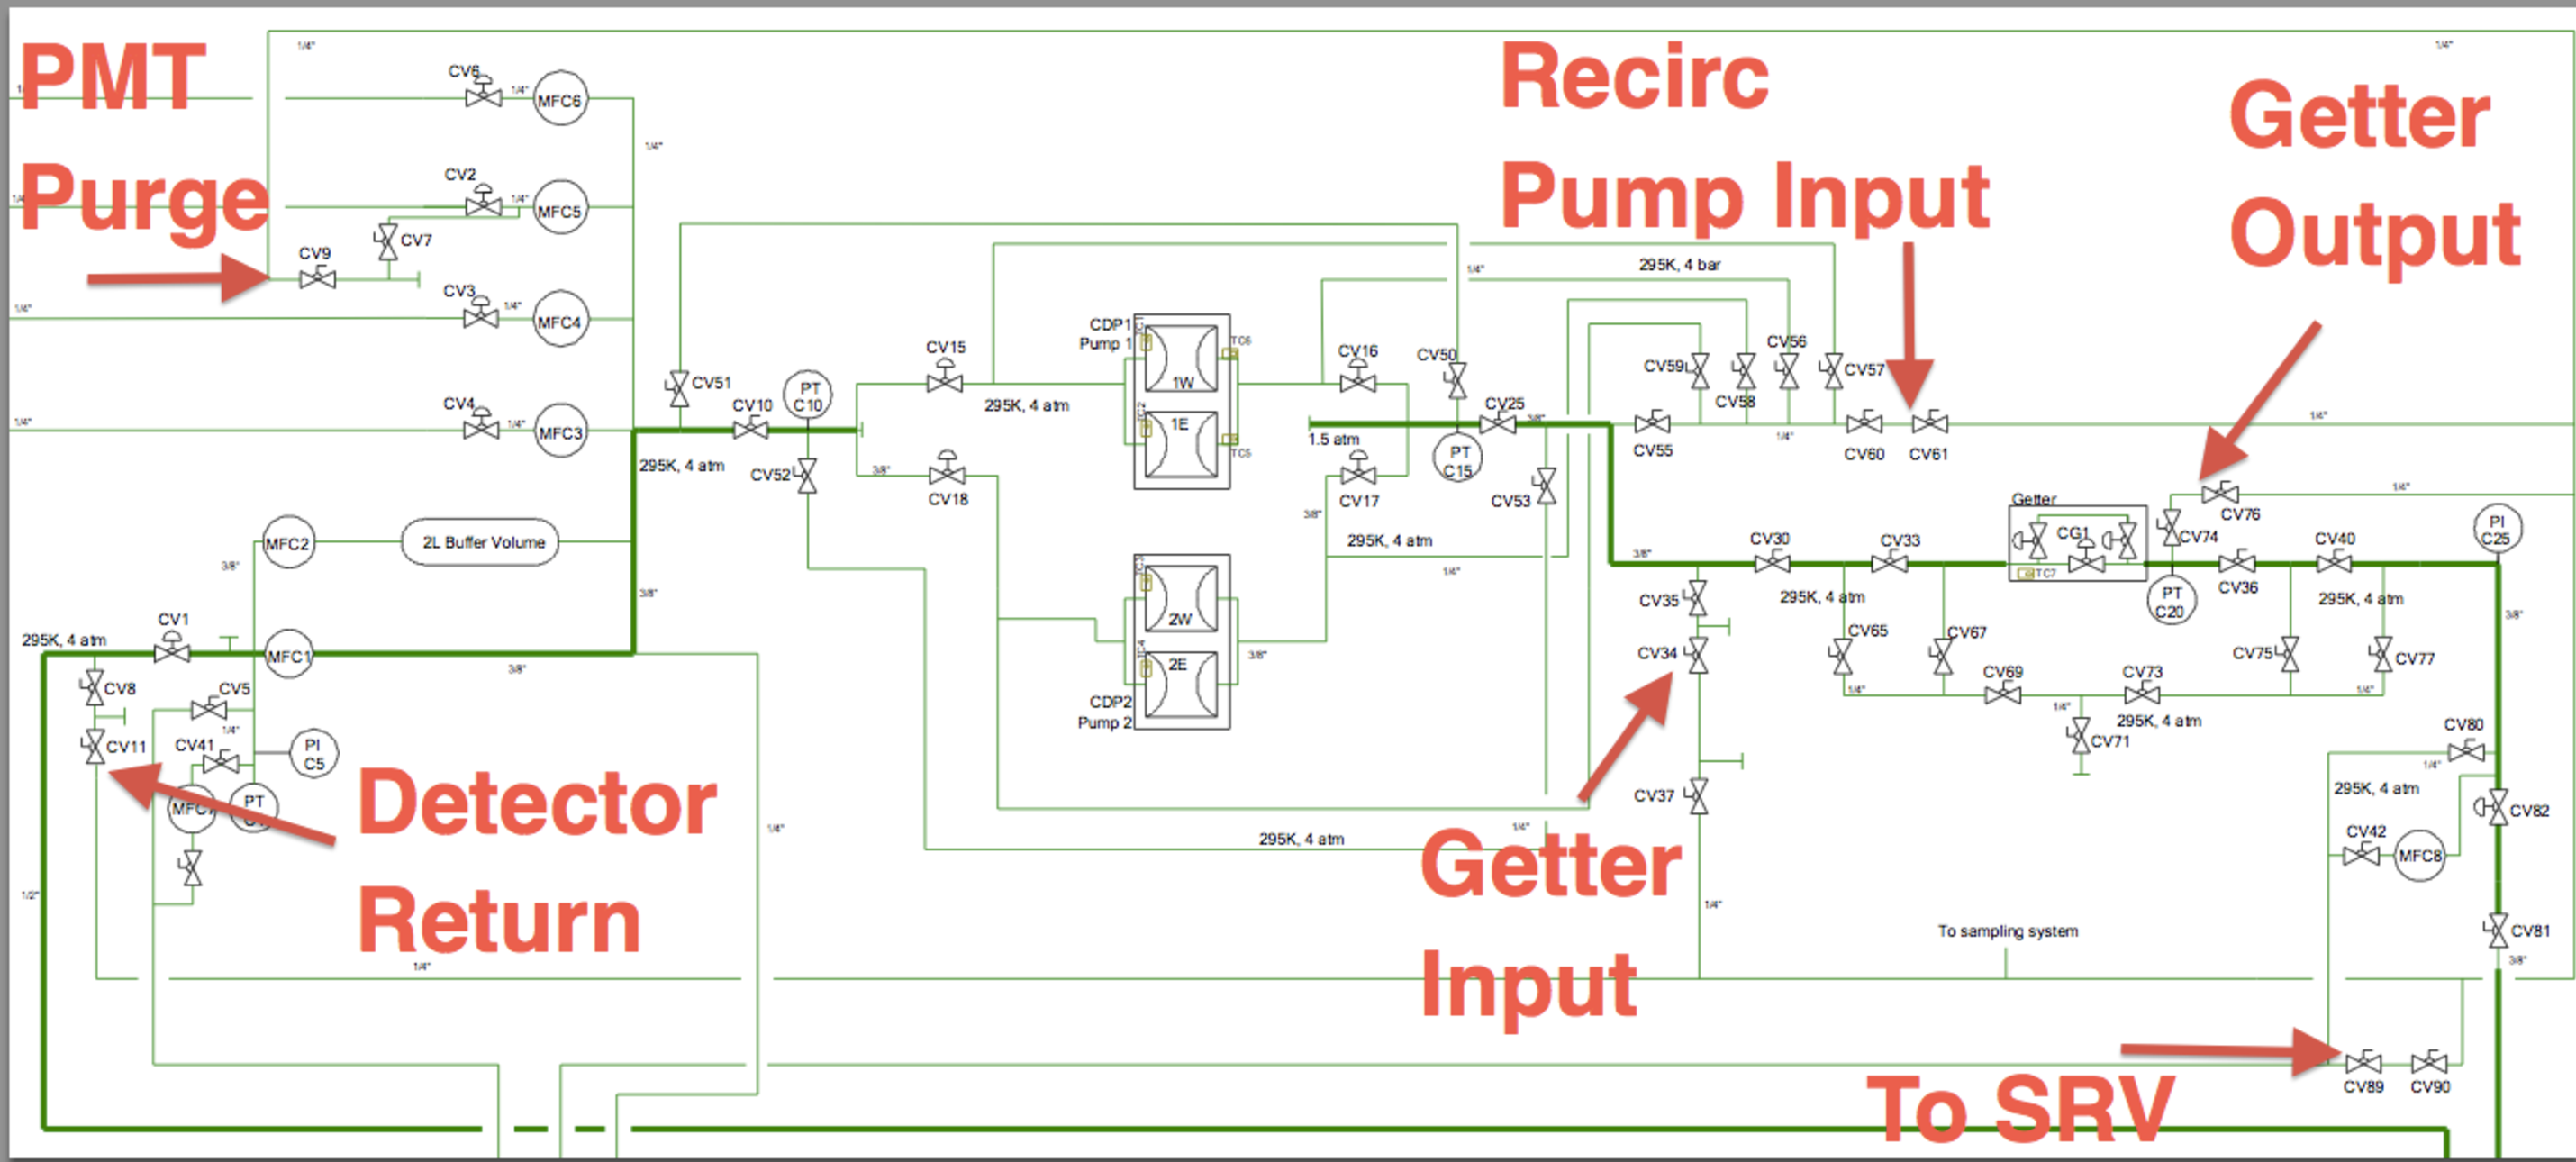
\includegraphics[width=150mm]{SamplingLocations.pdf}
\caption{Sampling Locations}
\label{fig:ports}
\end{figure}

\begin{figure}[h!]\centering
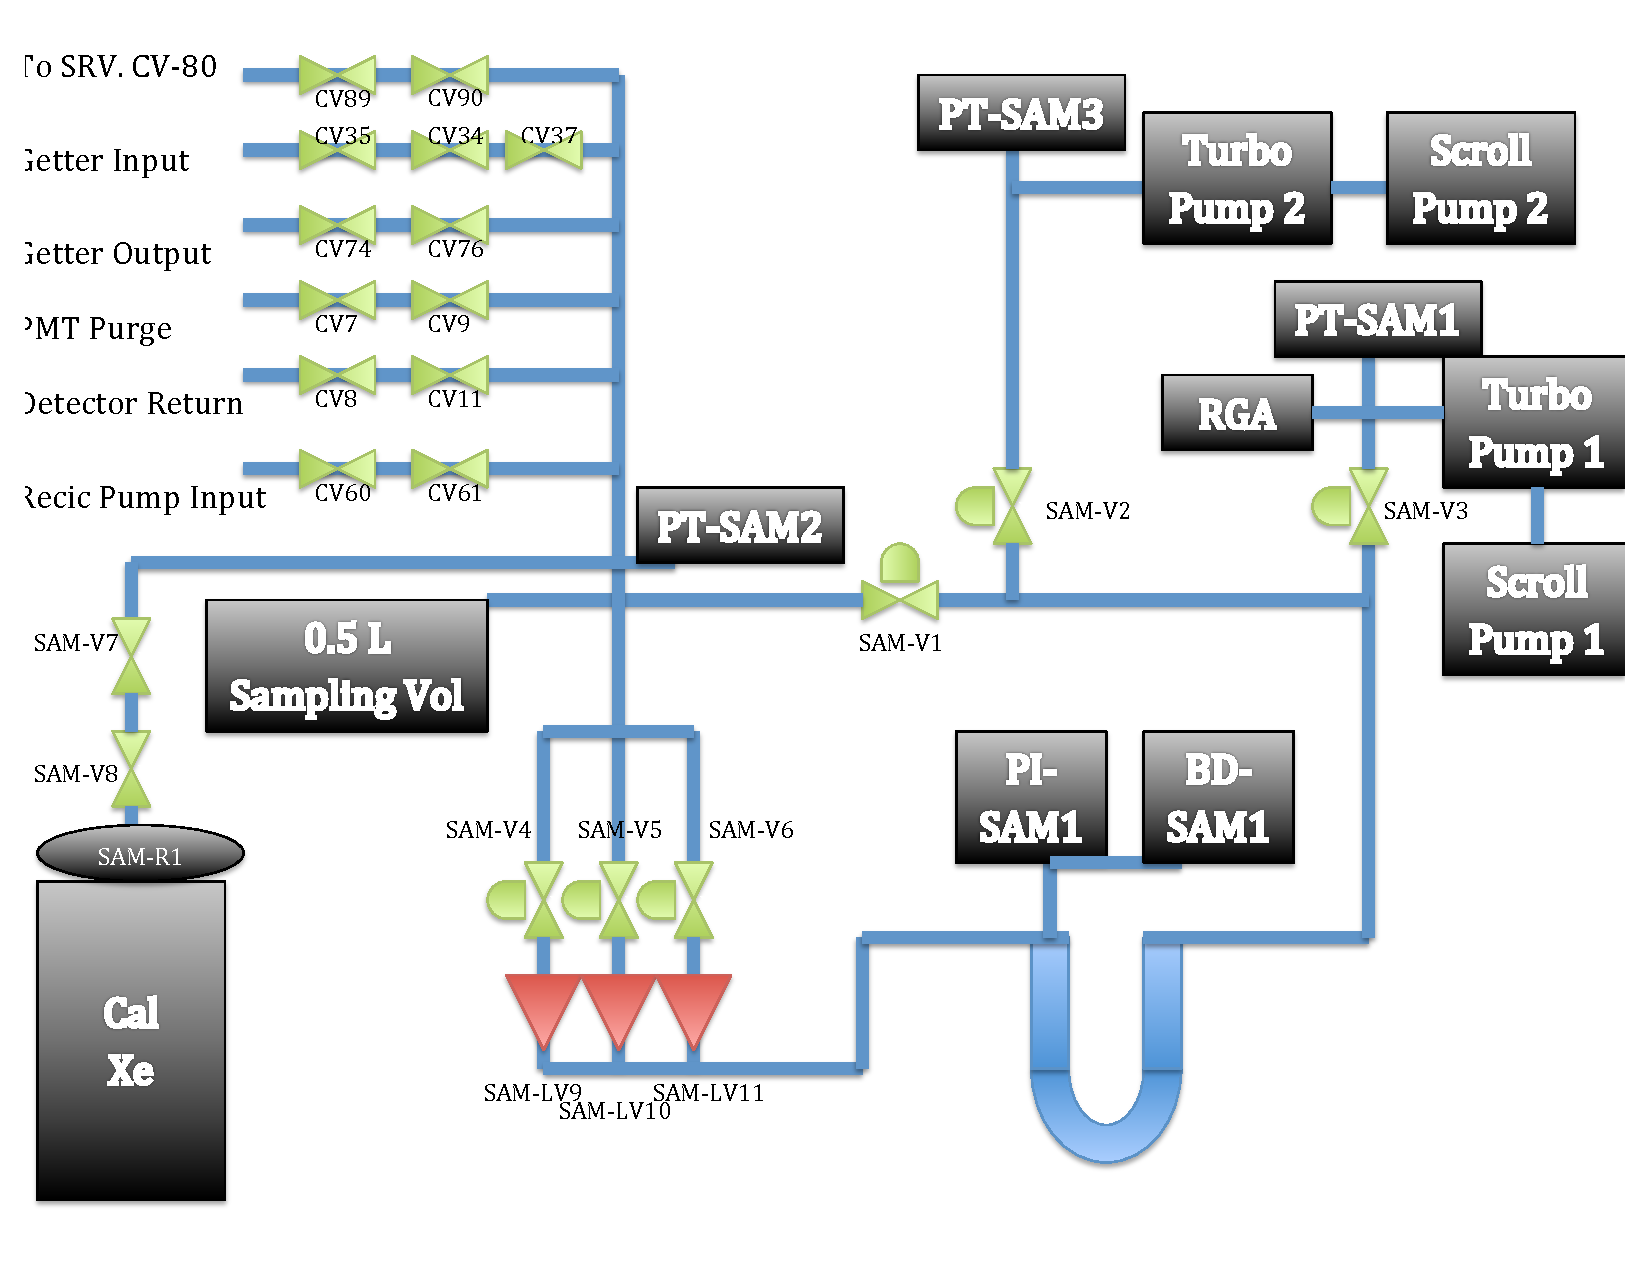
\includegraphics[width=150mm]{SAM_Diagram.pdf}
\caption{Diagram of the Coldtrap Sampling System}
\label{fig:pid}
\end{figure}

\begin{figure}[h!]\centering
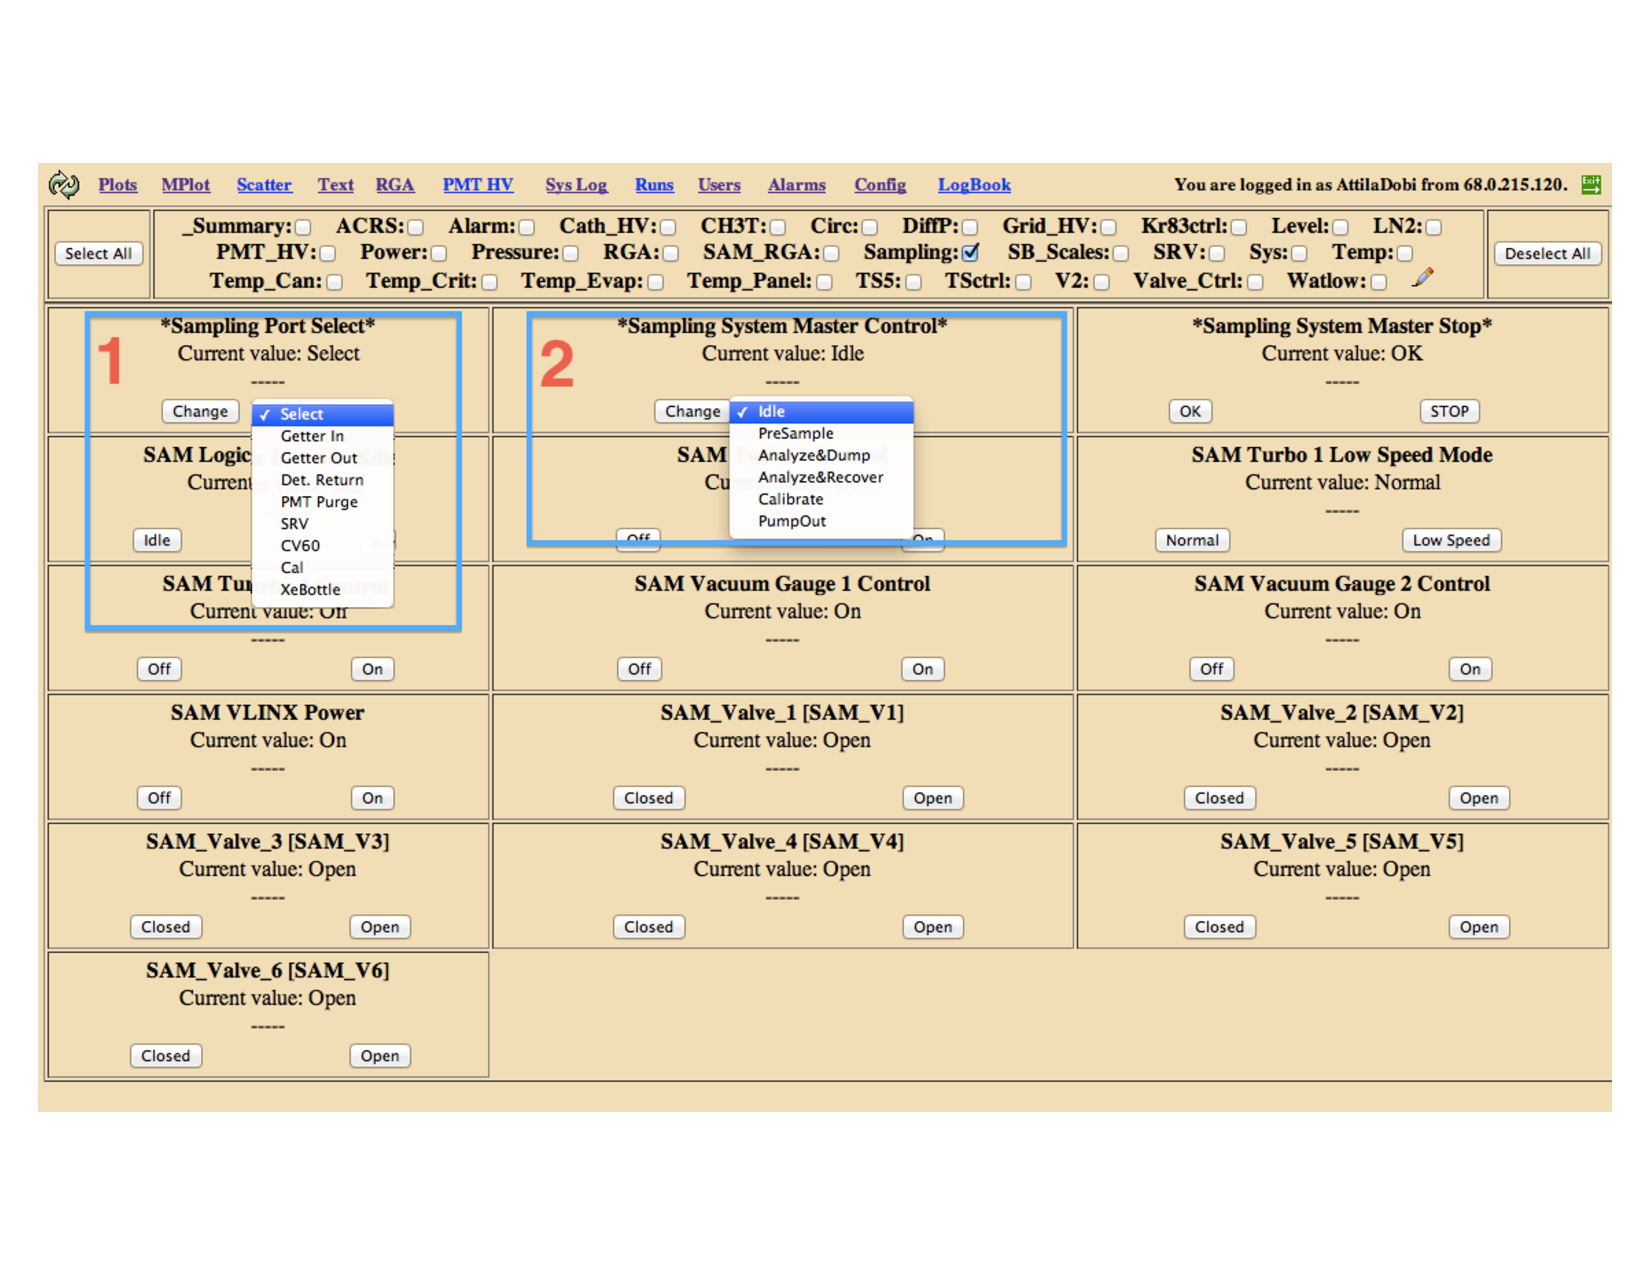
\includegraphics[width=150mm]{SAM_CTRL.pdf}
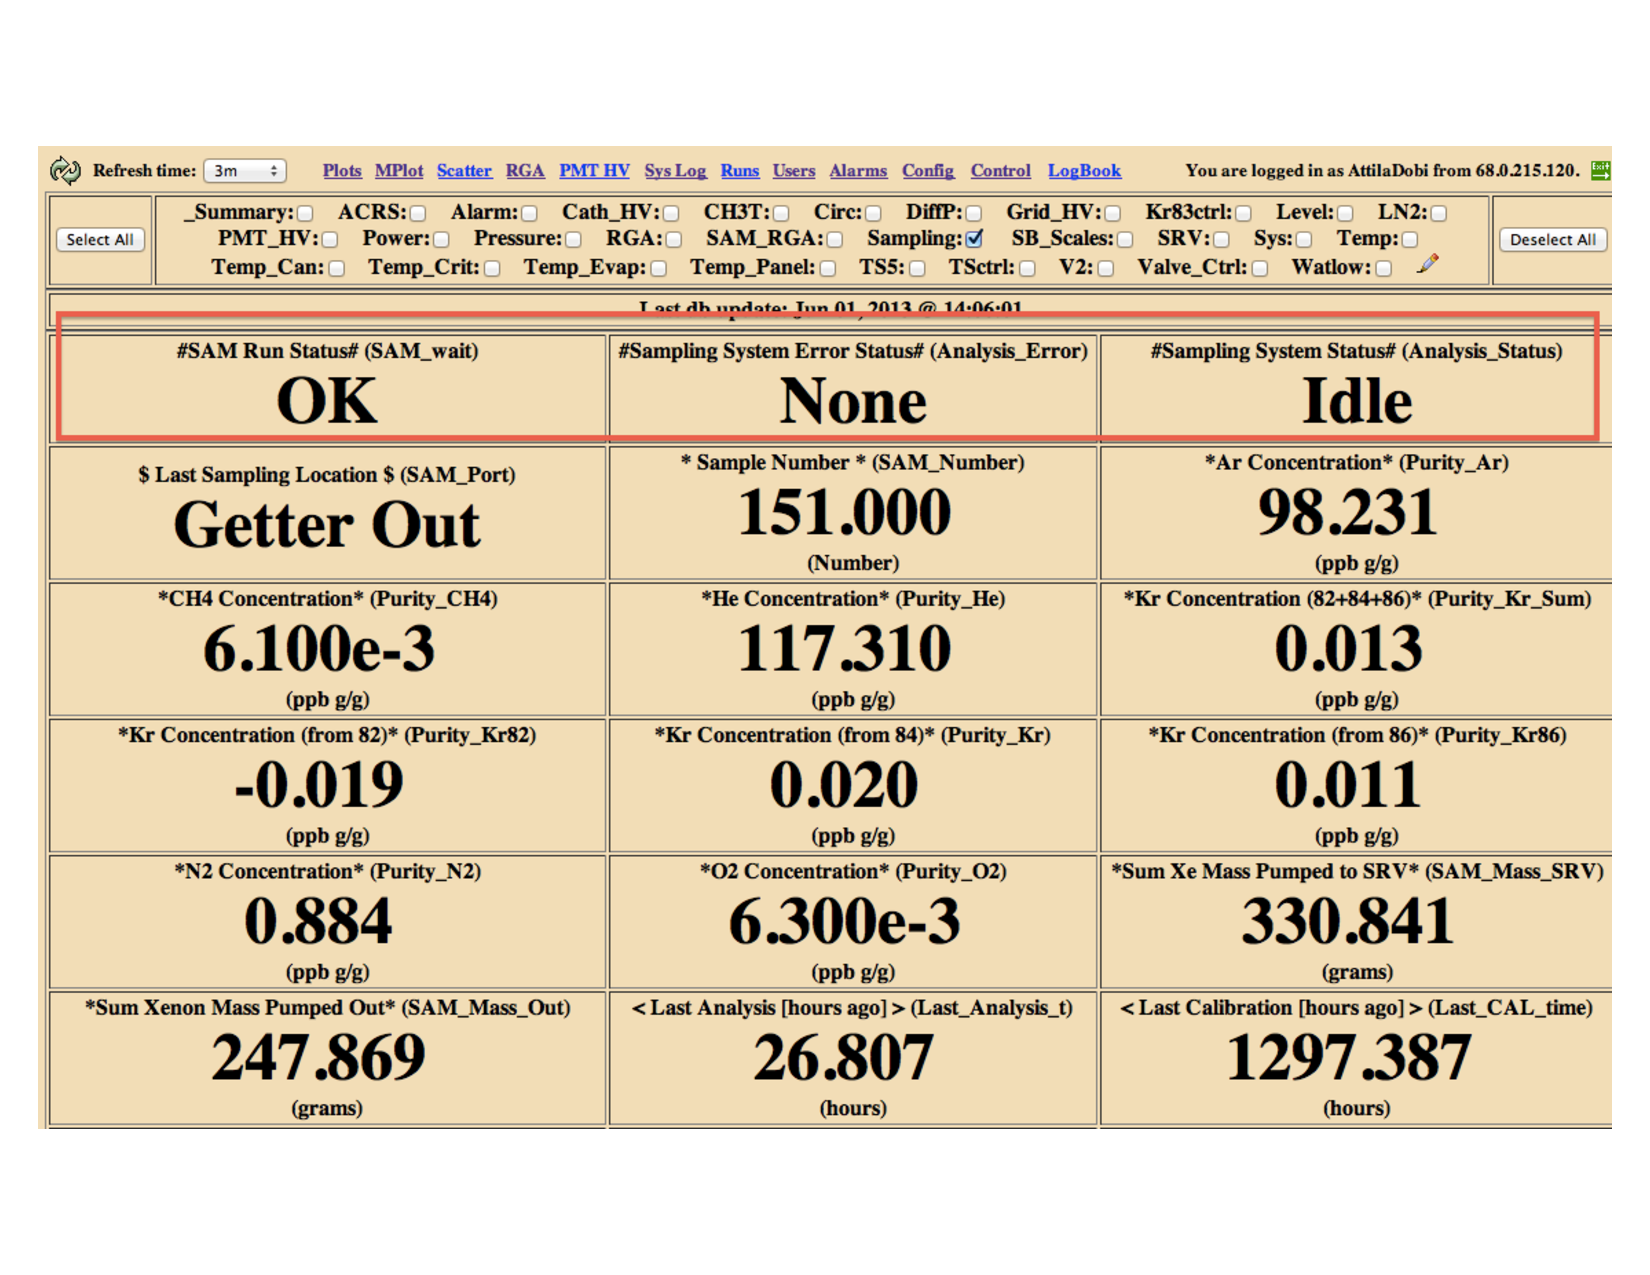
\includegraphics[width=150mm]{SAM_Status.pdf}
\caption{Top: The Sampling System Master Control box in LUX slow control. Bottom: The Sampling System status display in LUX slow control}
\label{fig:SC}
\end{figure}

\begin{figure}[h!]\centering
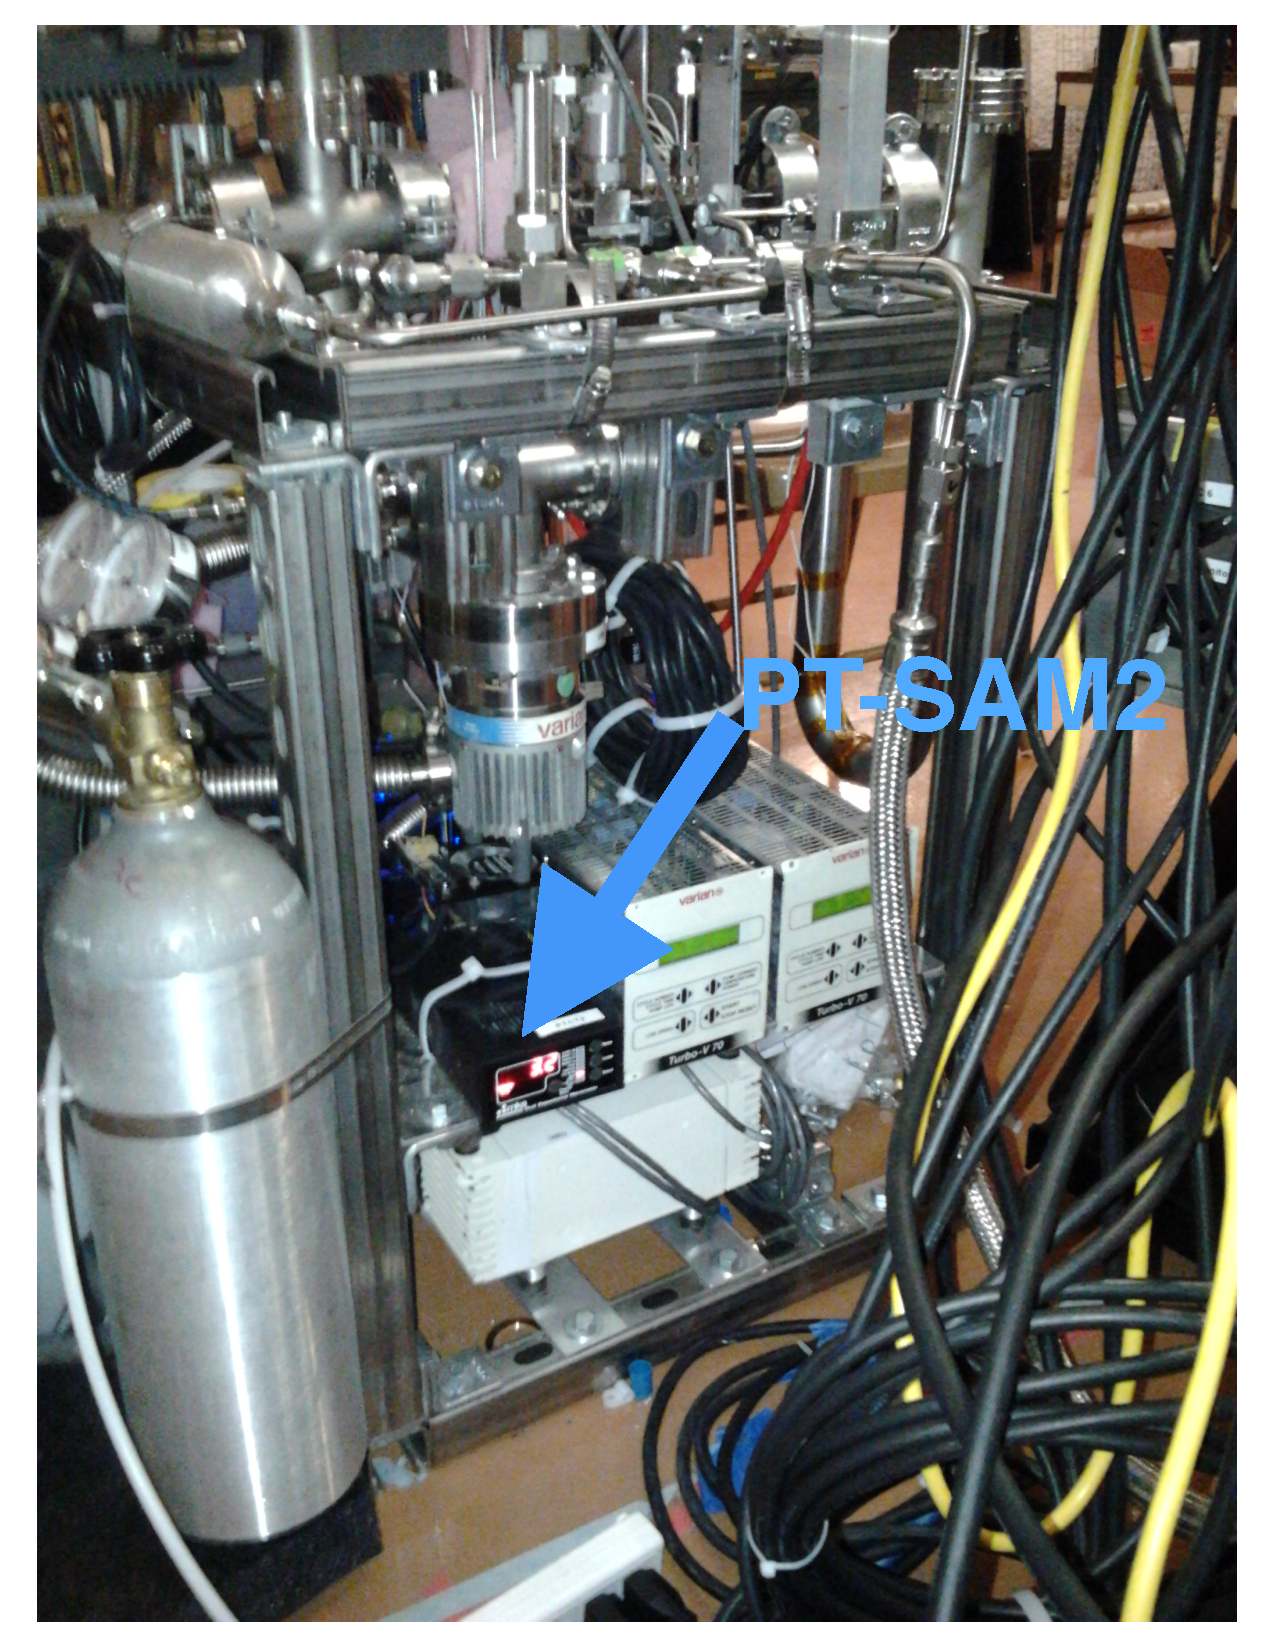
\includegraphics[width=100mm]{SAM.pdf}
\caption{The view of the sampling system from behind the circulation panel, where the xenon samples will be drawn. The user should watch PT-SAM2 when drawing a xenon sample.}
\label{fig:CM}
\end{figure}


\begin{figure}[h!]\centering
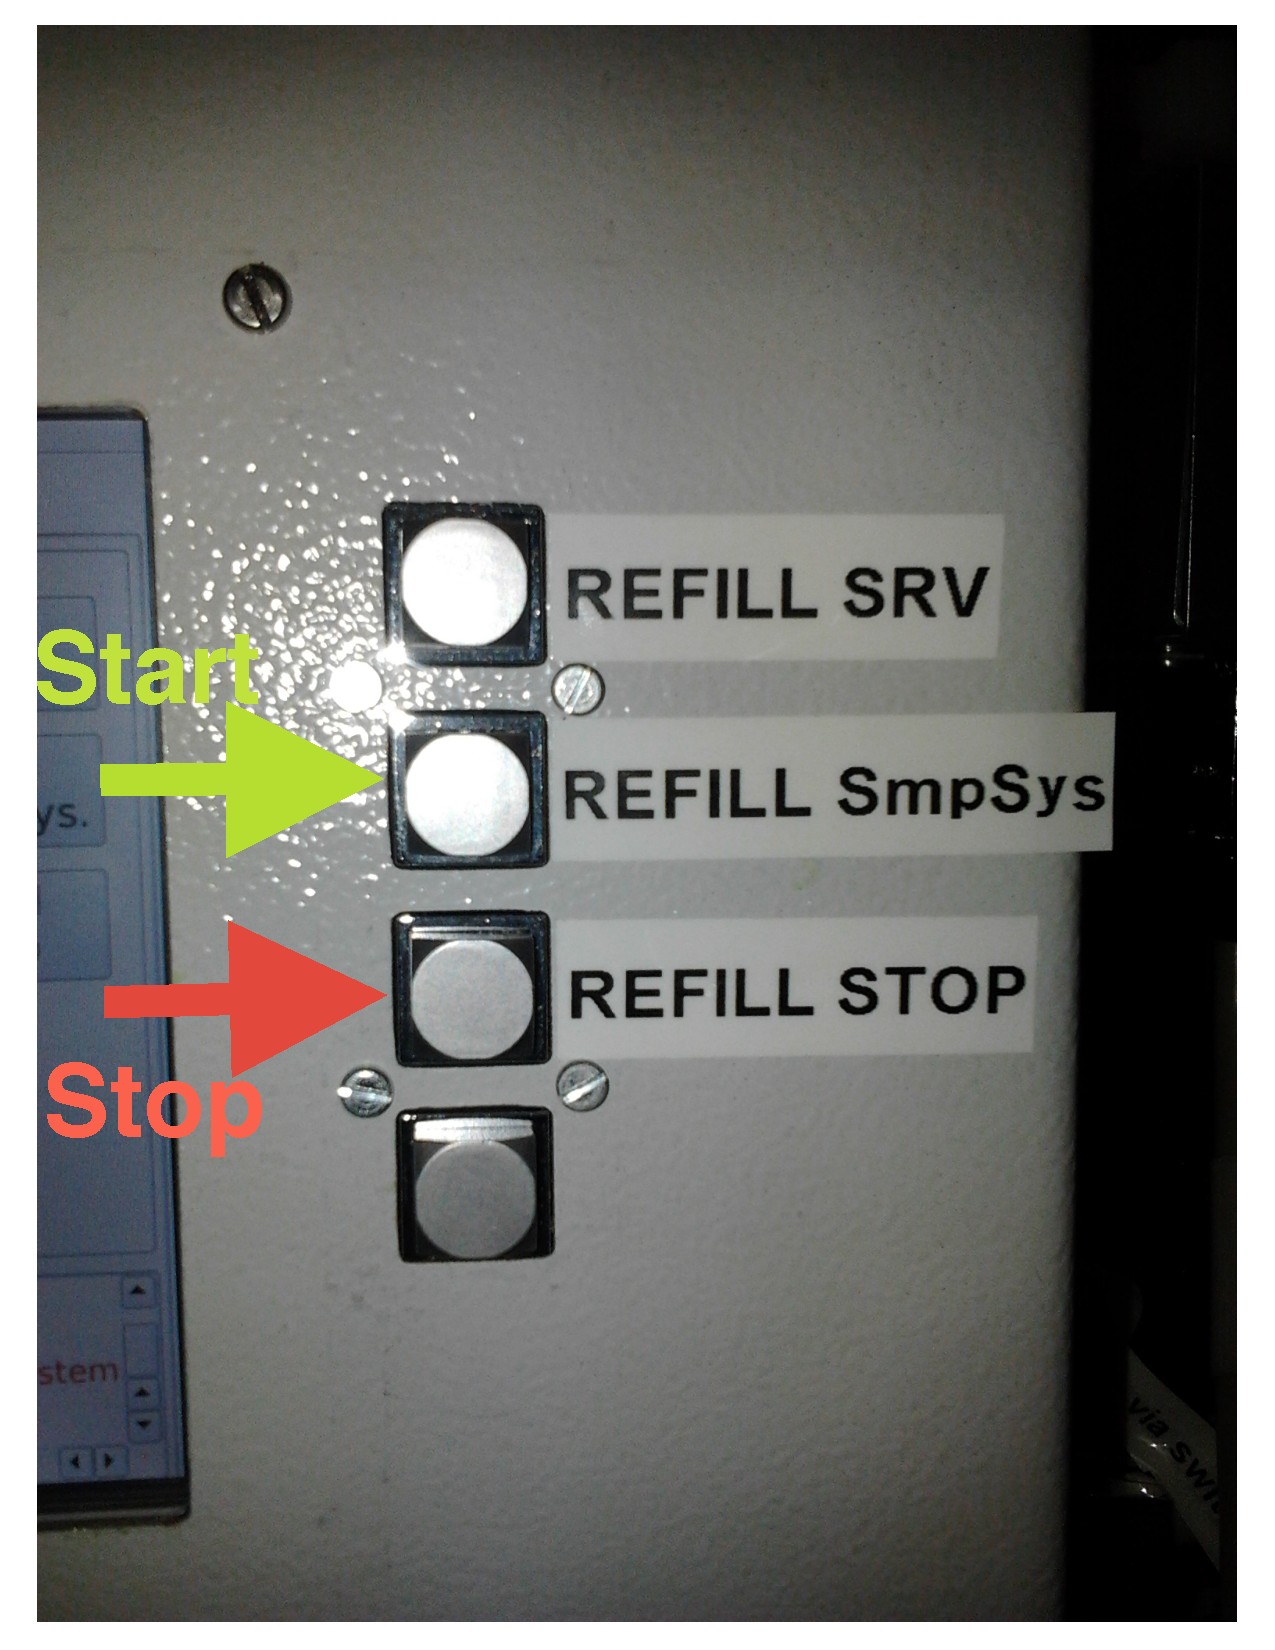
\includegraphics[width=100mm]{SRV_LN_BOX.pdf}
\caption{SRV LN system control box. To fill the 4 L transfer dewar push ``Refill SmsSys" to begin the flow of LN through the SRV pre-cool line. Once the dewar is full hit the ``Refill STOP" button.}
\label{fig:LN_BOX}
\end{figure}


\begin{figure}[h!]\centering
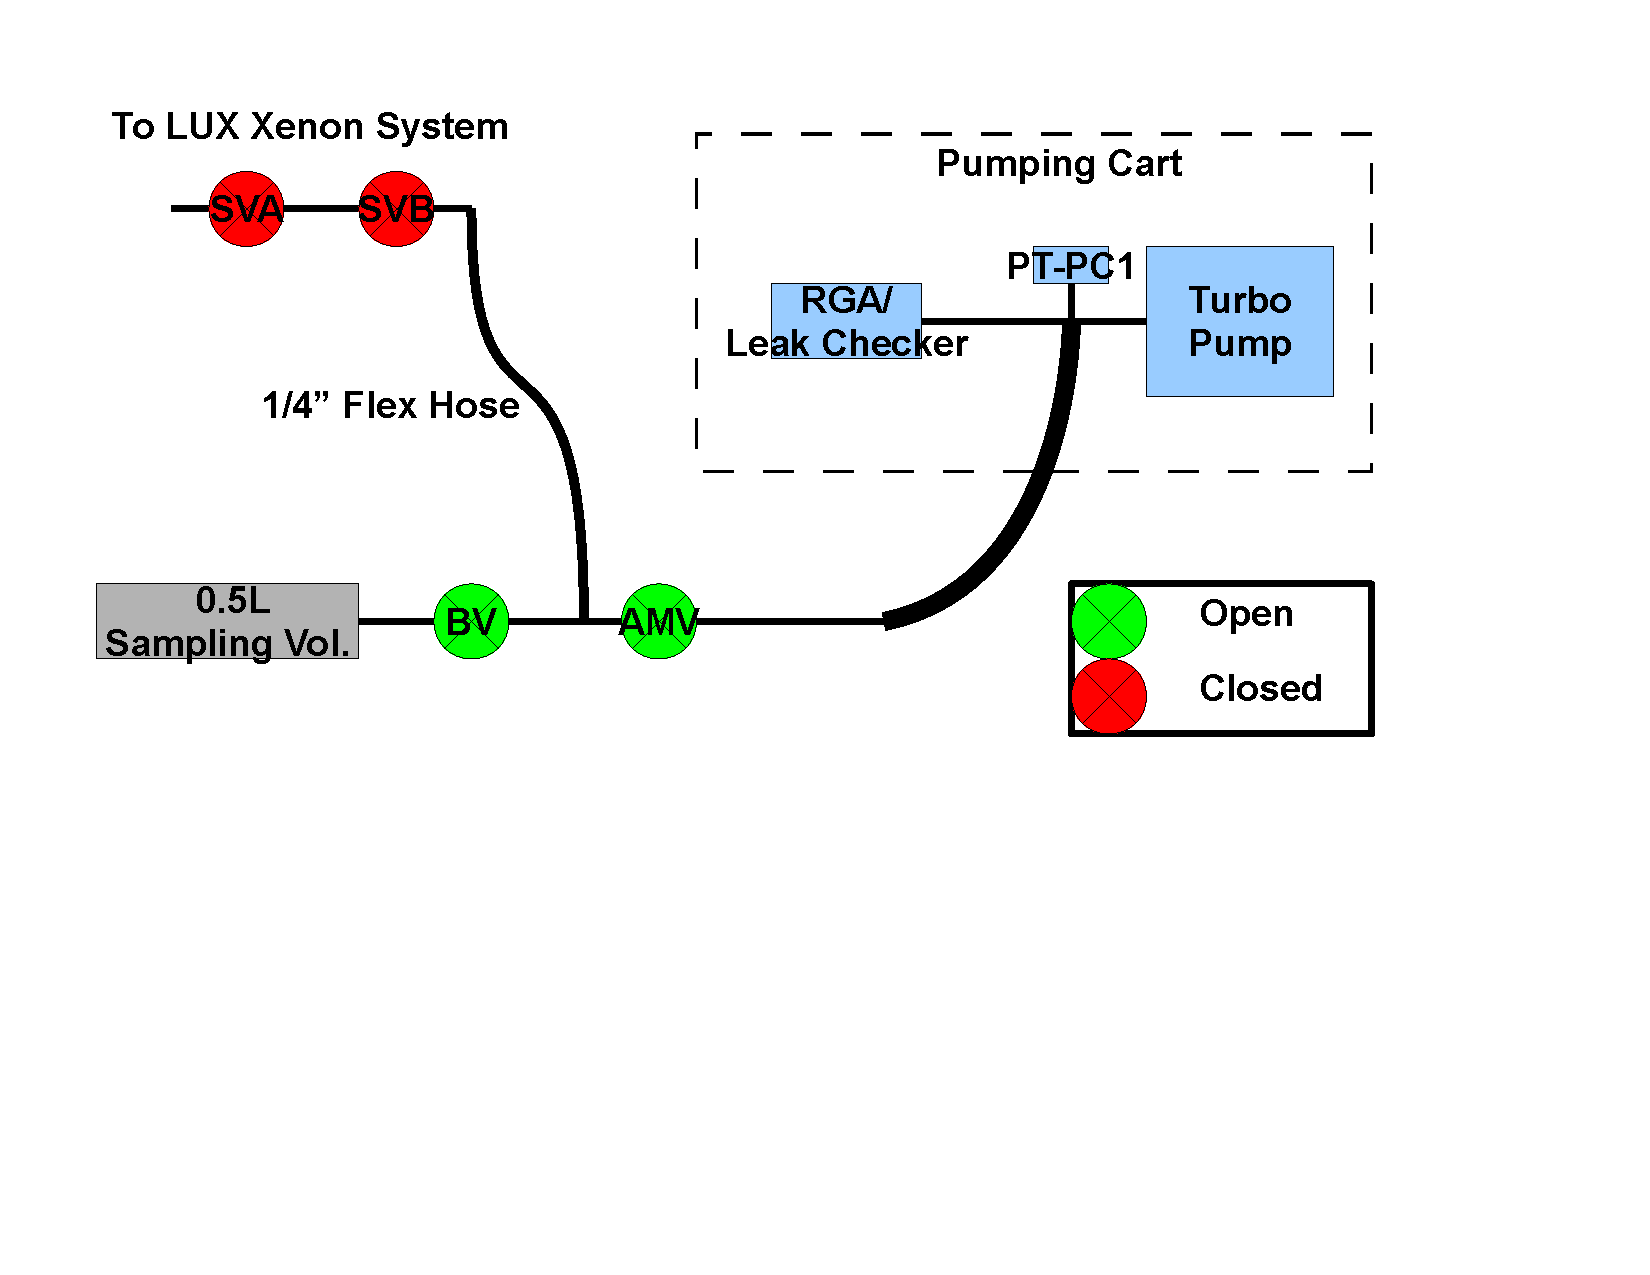
\includegraphics[width=150mm]{11.pdf}
\caption{Illustrated procedure for attaching the sampling manifold to the LUX xenon system}
\label{fig:fig2}
\end{figure}

\begin{figure}[h!]\centering
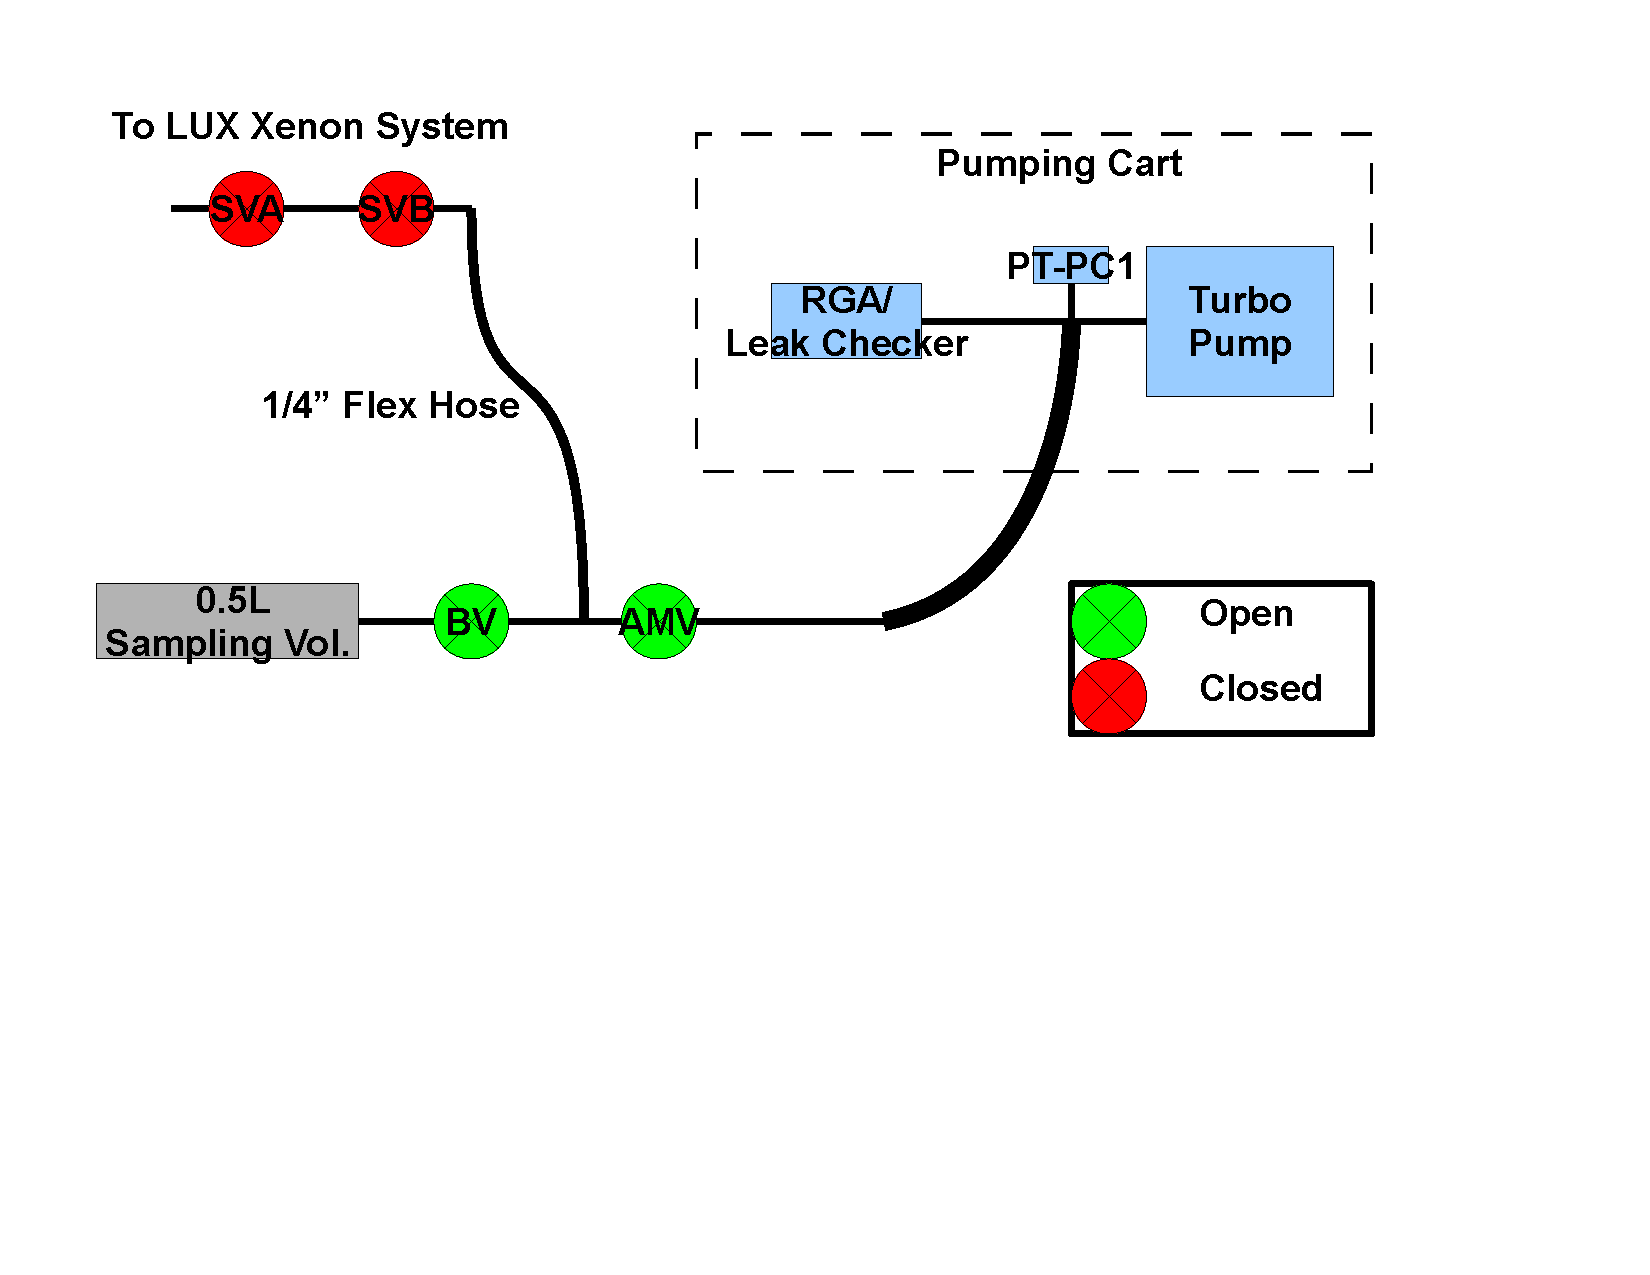
\includegraphics[width=80mm]{11.pdf}
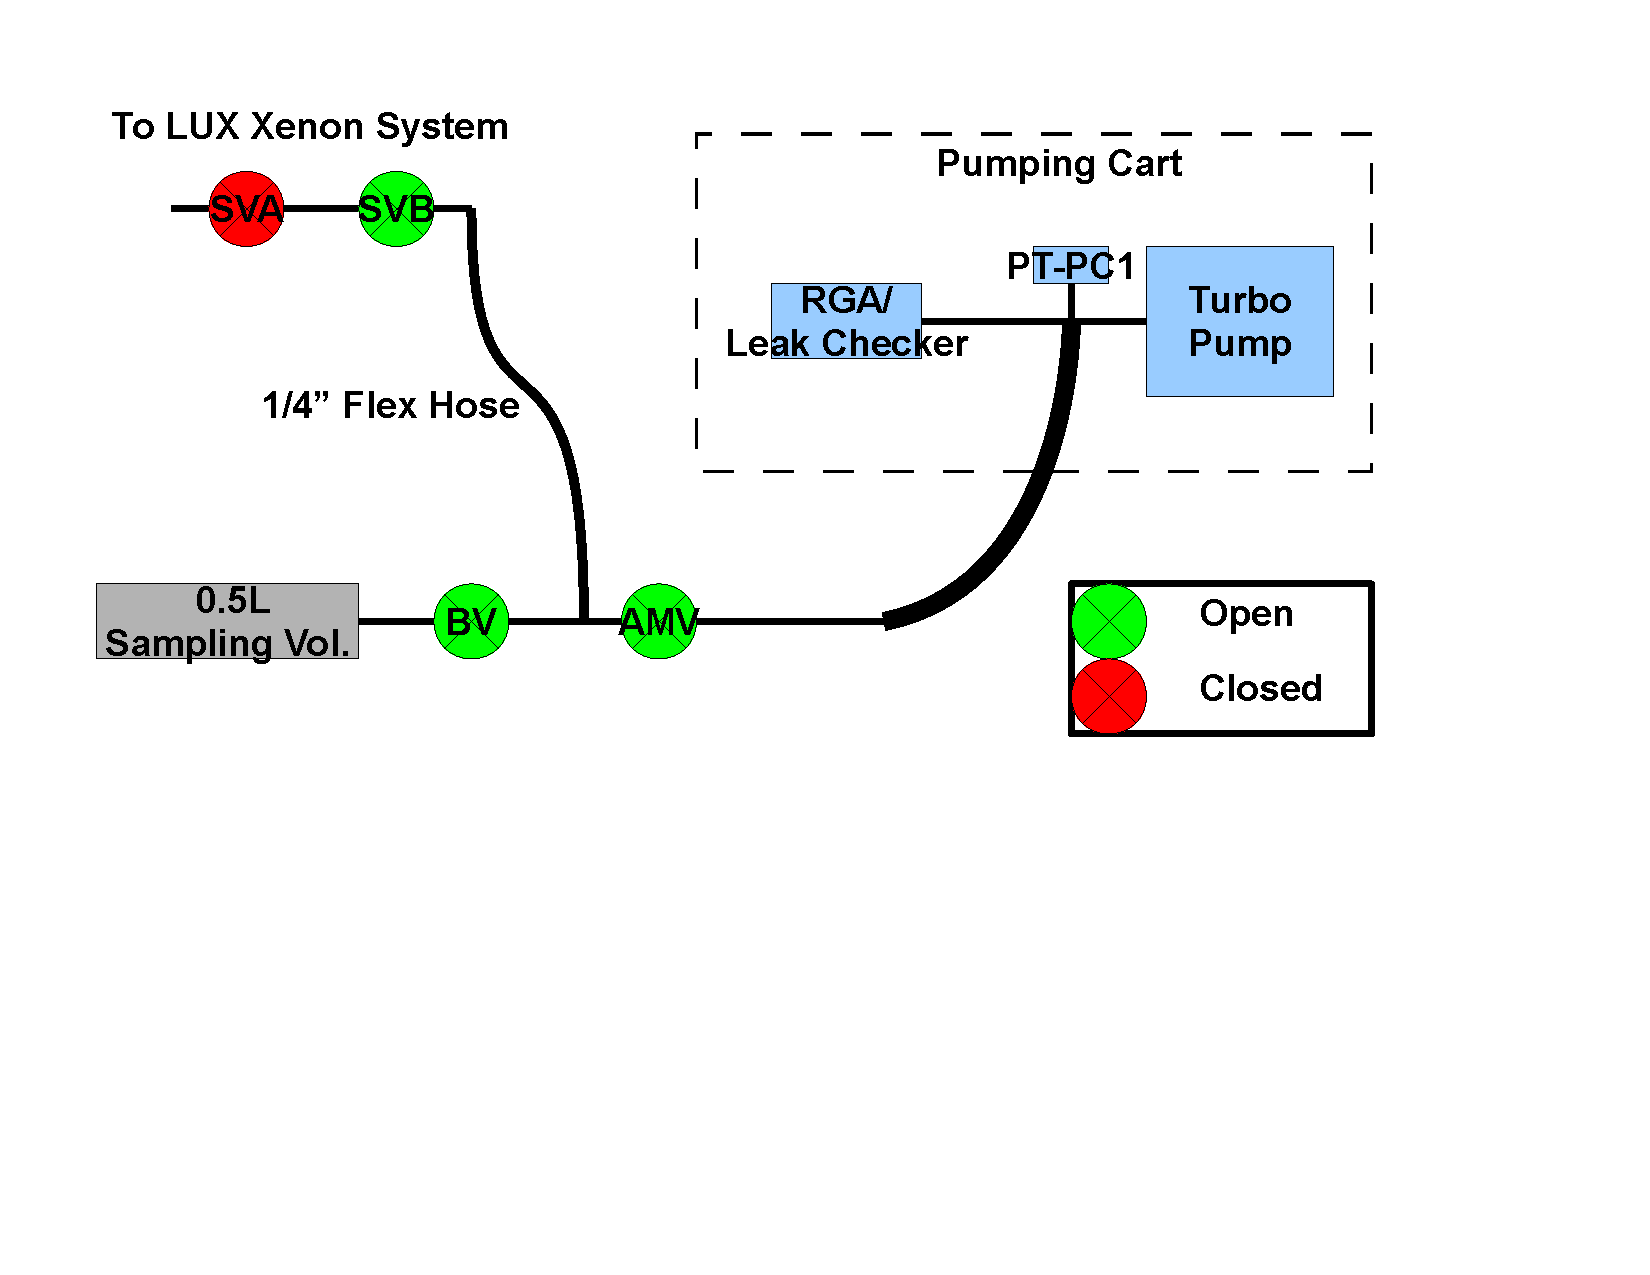
\includegraphics[width=80mm]{22.pdf}
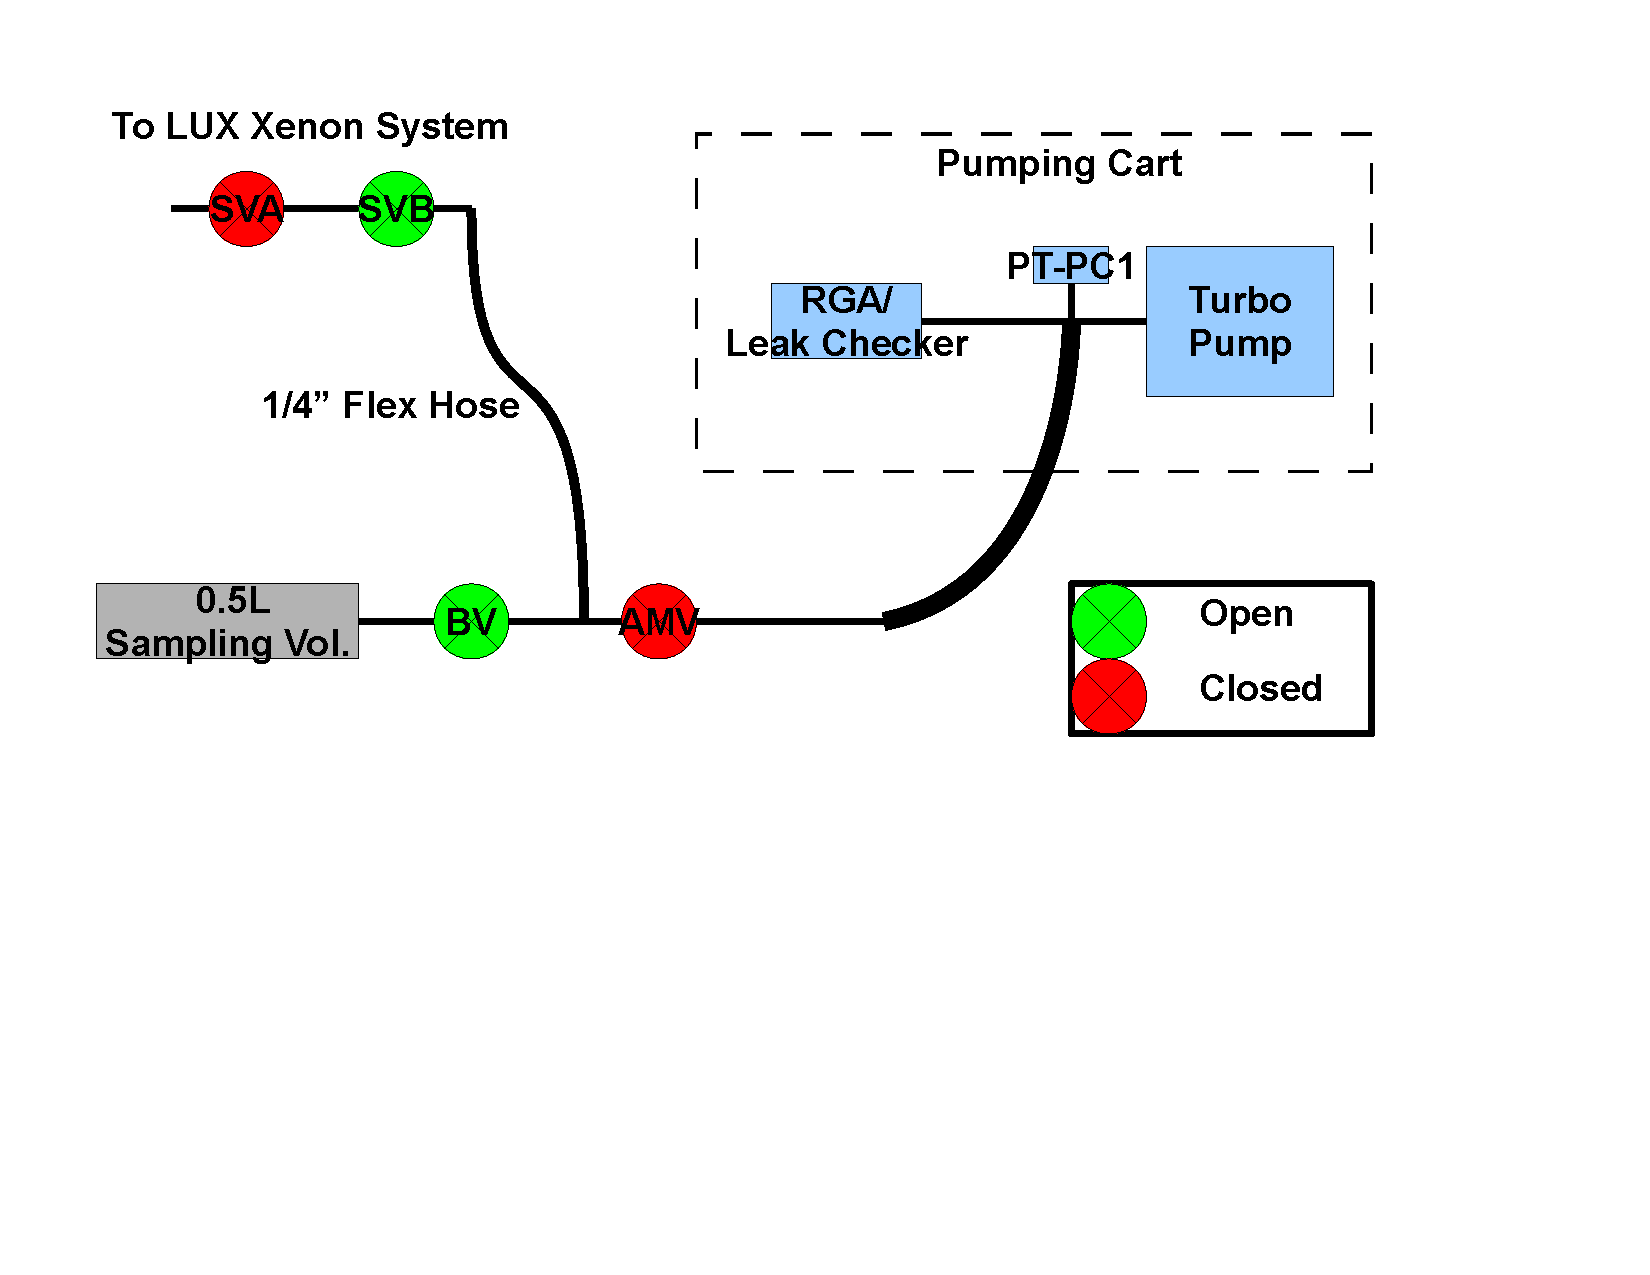
\includegraphics[width=80mm]{33.pdf}
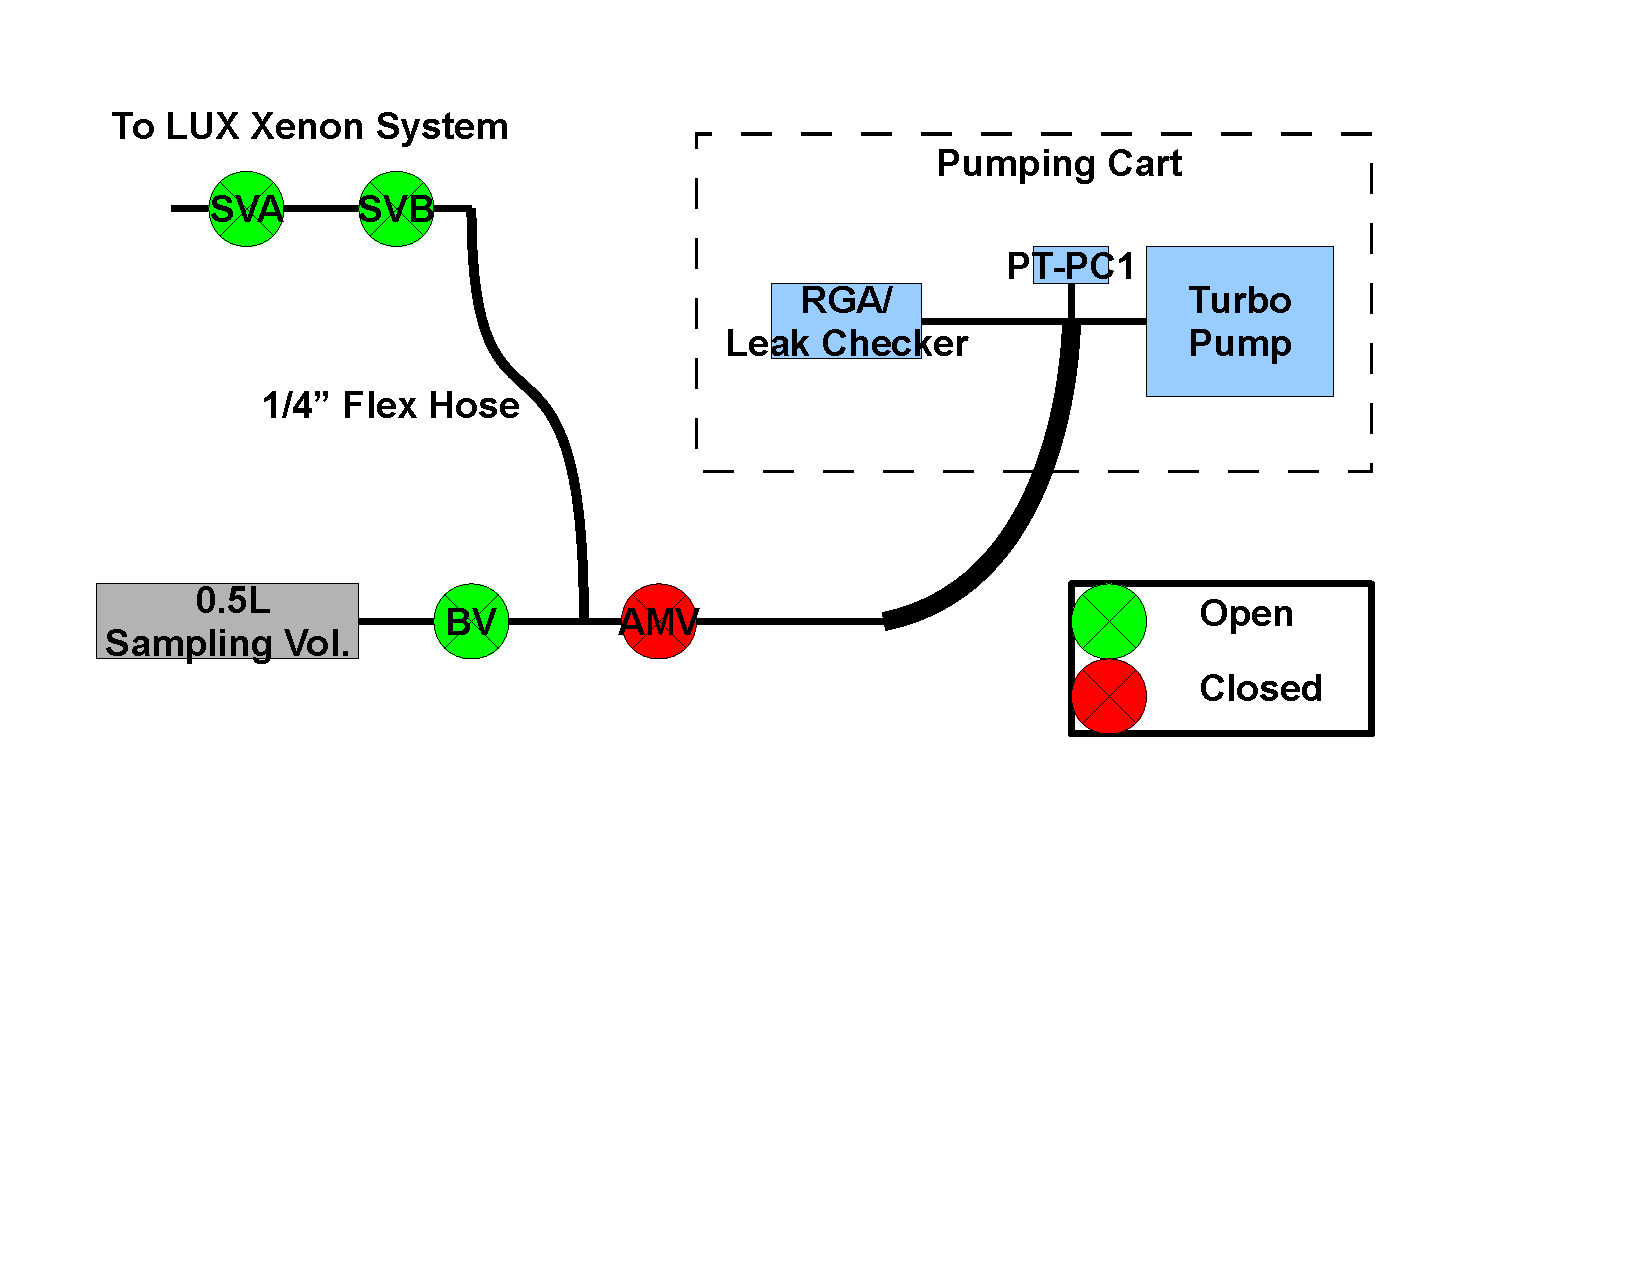
\includegraphics[width=80mm]{44.pdf}
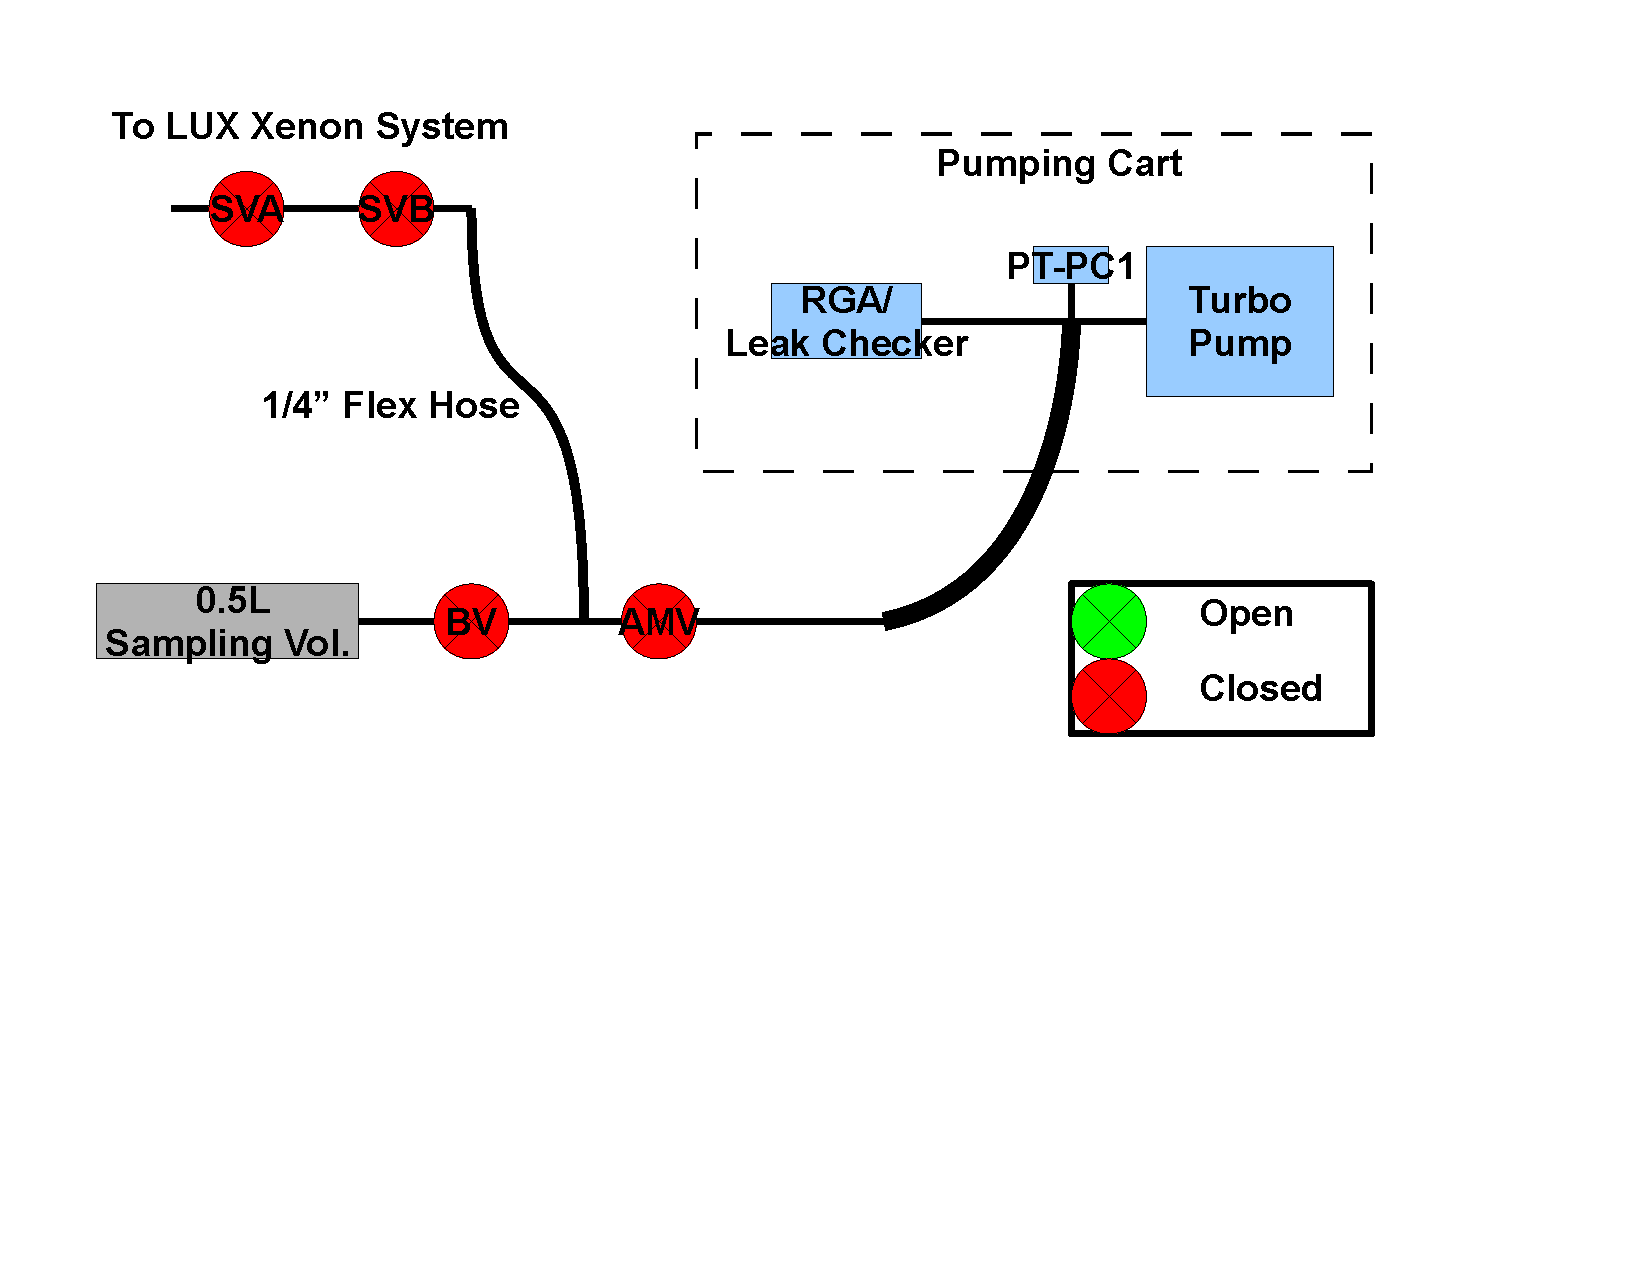
\includegraphics[width=80mm]{55.pdf}
\caption{Illustrated procedure for filling the sample bottle. First(top left), the sampling plumbing is attached to VB and then pumped to vacuum with the scroll-pump on the pumping cart. Second(top right), once the pressure on PT-PC1 reaches less than 0.1Torr VB is opened. The plumbing up to VA is then pumped to vacuum with the turbo-pump for one hour. Third(middle left), after pumping to vacuum for one hour the turbo-pump cart is isolated by closing AMV. Fourth(middle right), VA is opened filling the 0.5 L sample bottle with xenon at system pressure. Fifth(bottom), the VA, VB and the sample-bottle's valve (BV) are closed.}
\label{fig:steps}
\end{figure}




\end{document}
